\documentclass[sigconf,review,anonymous]{acmart}

\AtBeginDocument{%
  \providecommand\BibTeX{{%
    Bib\TeX}}}

% RecSys 2026 submission mode (anonymous review).
% For camera-ready, switch documentclass to [sigconf] and replace rights metadata
% below with the exact values from ACM rights management.
\setcopyright{none}
\acmConference[RecSys '26]{Proceedings of the 20th ACM Conference on Recommender Systems}{September 28--October 2, 2026}{Minneapolis, MN, USA}
\acmBooktitle{Proceedings of the 20th ACM Conference on Recommender Systems (RecSys '26), September 28--October 2, 2026, Minneapolis, MN, USA}
\acmDOI{}
\acmISBN{}

\usepackage{array}
\usepackage{dblfloatfix}
\usepackage{float}
\usepackage{makecell}
\usepackage{multirow}
\usepackage{placeins}
\usepackage{tabularx}
\usepackage[table]{xcolor}

\raggedbottom
\setlength{\emergencystretch}{2em}
\setcounter{topnumber}{3}
\setcounter{dbltopnumber}{2}
\renewcommand{\topfraction}{0.9}
\renewcommand{\dbltopfraction}{0.9}
\renewcommand{\textfraction}{0.07}
\renewcommand{\floatpagefraction}{0.8}
\renewcommand{\dblfloatpagefraction}{0.8}
\setlength{\textfloatsep}{10pt plus 2pt minus 2pt}
\setlength{\dbltextfloatsep}{9pt plus 2pt minus 2pt}
\setlength{\floatsep}{8pt plus 2pt minus 2pt}
\setlength{\dblfloatsep}{8pt plus 2pt minus 2pt}
\setlength{\intextsep}{8pt plus 2pt minus 2pt}

\newcolumntype{Y}{>{\centering\arraybackslash}X}
\newcolumntype{L}[1]{>{\raggedright\arraybackslash}p{#1}}
\definecolor{routerecgray}{RGB}{242,242,242}
\newcommand{\tblbest}[1]{\textbf{#1}}
\newcommand{\tblsecond}[1]{\underline{#1}}
\newcommand{\placeholderpanel}[1]{\fbox{\rule{0pt}{#1}\rule{0.92\linewidth}{0pt}}}

\begin{document}

\title[RouteRec for Sequential Recommendation]{RouteRec: Behavior-Guided Sparse Routing for Sequential Recommendation}

\author{First Author}
\affiliation{%
  \institution{KAIST}
  \department{Kim Jaechul Graduate School of AI}
  \city{Daejeon}
  \country{Republic of Korea}}
\email{first.author@kaist.ac.kr}

\author{Second Author}
\affiliation{%
  \institution{KAIST}
  \department{Kim Jaechul Graduate School of AI}
  \city{Daejeon}
  \country{Republic of Korea}}
\email{second.author@kaist.ac.kr}

\renewcommand{\shortauthors}{Author et al.}

\begin{abstract}
Sequential recommendation exhibits heterogeneous behavioral regimes, yet most models still process all prefixes through largely shared computation. In practice, some prefixes are governed by stable preference, others by evolving session intent, and others by immediate local transitions. This creates a mismatch between behavioral diversity and shared computation. Mixture-of-experts (MoE) offers a natural mechanism for conditional computation, but hidden-state-driven routing remains limited for this setting: it is often semantically opaque, and dense expert mixing weakens commitment to behavior-specific computation paths.

We propose \textbf{RouteRec}, a behavior-guided sparse conditional computation framework for sequential recommendation built around three principles. First, RouteRec derives \emph{portable behavioral cues} from ordinary interaction logs, avoiding dependence on heavy side-information encoders. Second, it applies \emph{coarse-to-fine multi-stage routing} across macro, mid, and micro scopes so that long-range tendency, within-session evolution, and immediate transition cues can influence routing at different granularities. Third, it uses \emph{behavior-guided sparse expert allocation} that decouples routing signals from hidden representations and selectively activates only a subset of expert groups and experts at each stage.

This design treats behavior features as routing controls rather than as another representation-fusion channel. RouteRec therefore preserves strong sequence modeling in the representation path while introducing a compact, transferable control interface for conditional computation, with sharper route commitment and partial expert activation. Experiments show that RouteRec improves ranking quality on several datasets while remaining competitive on others, and yields more behavior-consistent routing patterns with reasonable efficiency in diagnostic analyses. Anonymous code: \url{https://anonymous.4open.science/r/RouteRec/}.
\end{abstract}

\begin{CCSXML}
<ccs2012>
 <concept>
  <concept_id>10002951.10003317.10003347.10003350</concept_id>
  <concept_desc>Information systems~Recommender systems</concept_desc>
  <concept_significance>500</concept_significance>
 </concept>
</ccs2012>
\end{CCSXML}

\ccsdesc[500]{Information systems~Recommender systems}

\keywords{sequential recommendation, sparse routing, conditional computation, routing, behavioral features}

\maketitle

\section{Introduction}
Sequential recommendation is usually formulated as next-item prediction over an ordered interaction history, but the underlying behavior is rarely homogeneous. Even for the same user, one prefix may reflect stable preference, another may reflect an evolving within-session goal, and another may be dominated by immediate local exploration. Prior work on sequential and session-based recommendation has repeatedly shown that user behavior mixes multiple regimes rather than following a single stationary pattern \cite{wang2019seqsurvey,wang2021sessionsurvey}.

Strong sequential recommenders model these histories increasingly well \cite{hidasi2016gru4rec,kang2018sasrec,li2020tisasrec,qiu2022duorec,shin2024bsarec,liu2025sigma}, yet they still process behaviorally different prefixes through largely shared computation. The result is a simple mismatch: heterogeneous behavior is acknowledged in the data, while computation remains mostly uniform.

Figure~\ref{fig:intro-behavioral-features} illustrates this gap. Distinct users and sessions can differ in pace, repetition, focus, and local transition patterns, yet standard sequential models expose limited control over how such differences should change the computation path. Existing advances therefore improve representation quality, but they leave the allocation of computation mostly implicit.

\begin{figure}[!t]
  \centering
  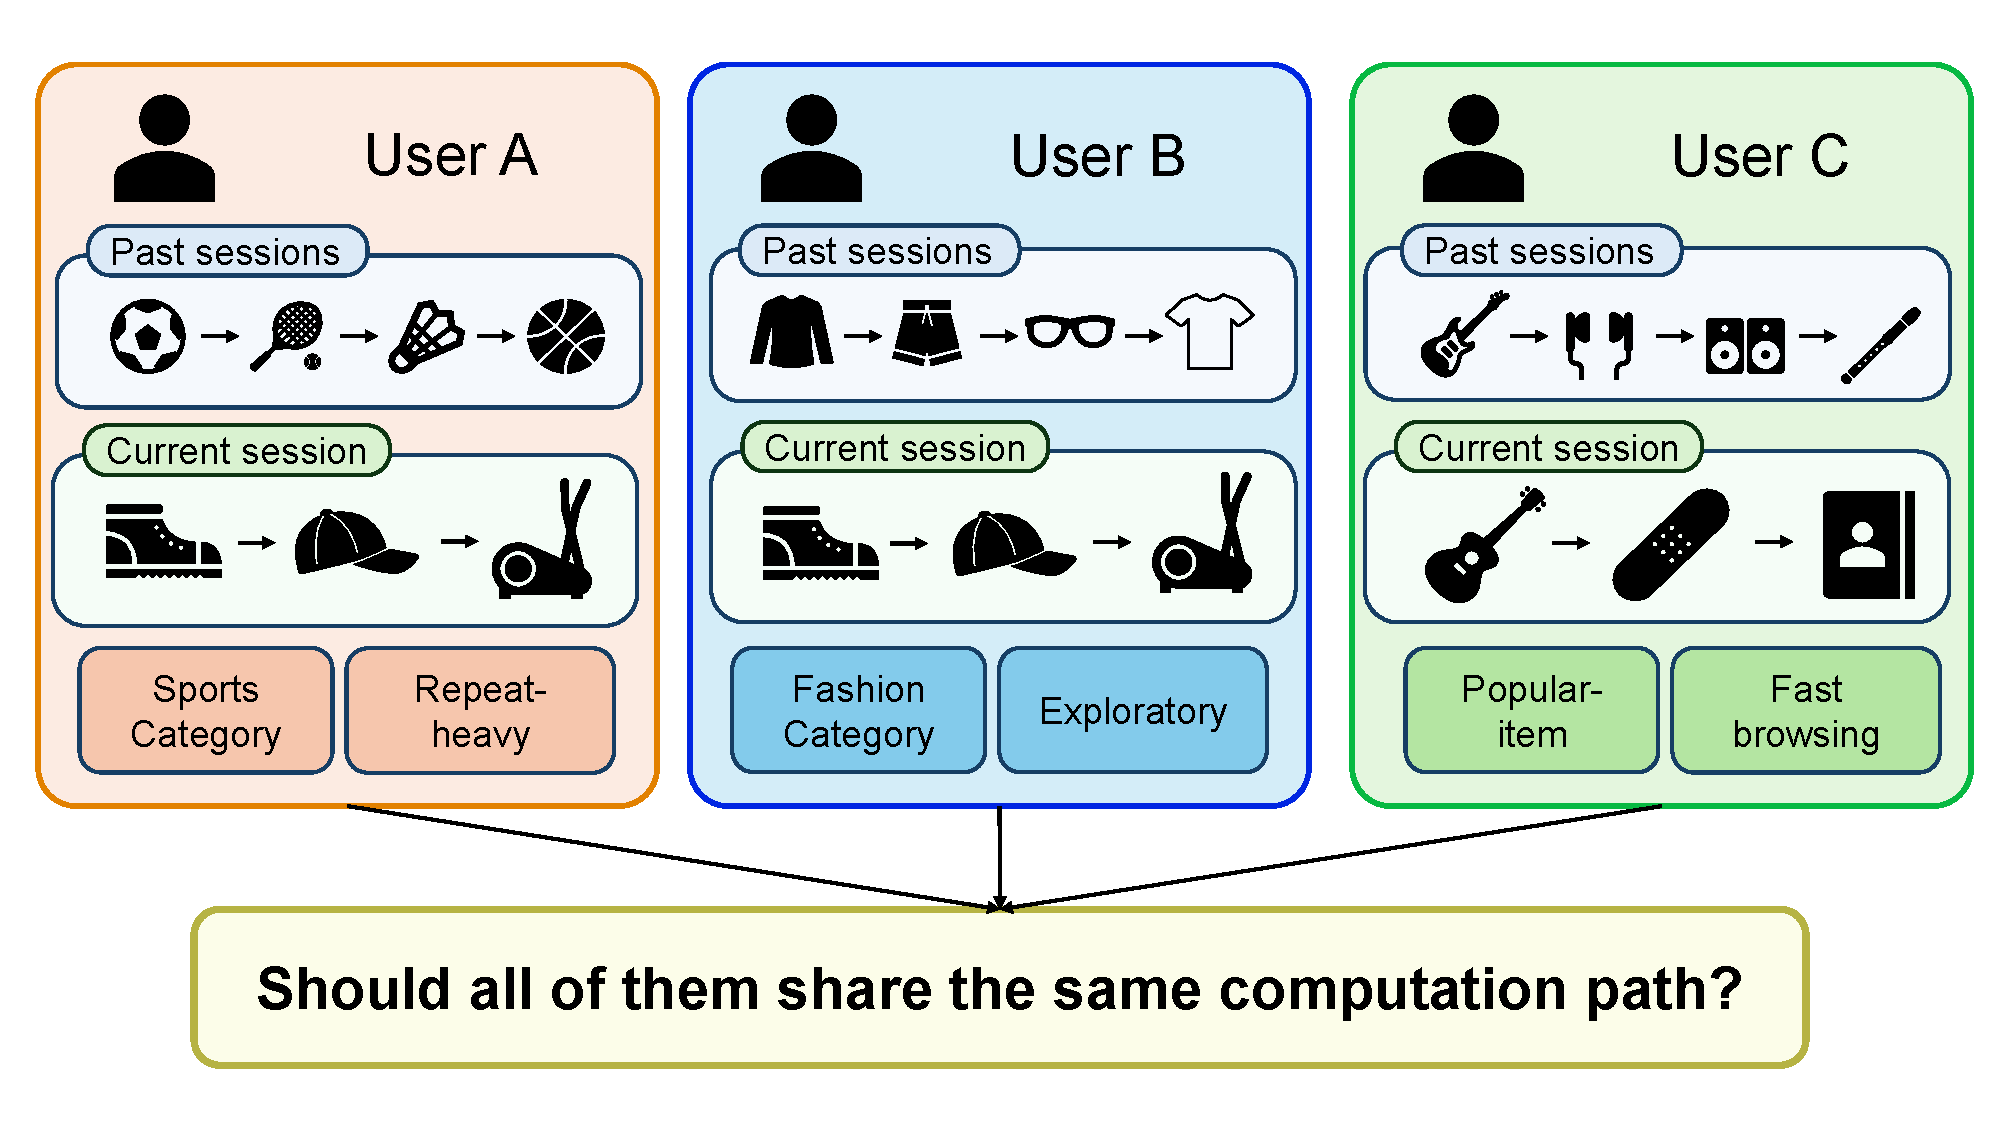
\includegraphics[width=\columnwidth]{figures/figure1_different_user.pdf}
  \caption{Different users and sessions can require different computational paths.}
  \Description{A problem-motivation figure contrasting different user and session behavior patterns, highlighting that behaviorally different cases are often processed with the same computation path in standard sequential recommendation.}
  \label{fig:intro-behavioral-features}
\end{figure}

Feature-aware and heterogeneity-aware sequential models partially address this issue, but mostly by enriching representations, reweighting attention, or decomposing interests within a shared computation pipeline. We ask a different question: can observable behavior cues control \emph{which computation path} should be used? Mixture-of-experts (MoE) is a natural candidate for this purpose \cite{jacobs1991adaptive,jordan1994hme,shazeer2017moe,fedus2022switch}, because it can replace one shared transformation with condition-dependent expert allocation. Yet simply inserting experts is not enough. If computation paths are meant to differ across behavioral regimes, the model should not only route differently, but also activate computation selectively. For sequential recommendation, routing must still answer why specialization is needed, where routing should differ across temporal evidence, what signals should drive routing in an interpretable way, and why sparse route commitment is preferable to a dense mixture over all experts.

\textbf{Challenge 1: behavioral diversity versus shared computation.} Real prefixes arise from different behavioral regimes, but most sequential recommenders still process them with largely shared computation. If routing is to be justified beyond generic extra capacity, it should be controlled by portable cues derived from ordinary logs rather than heavy dataset-specific side branches.

\textbf{Challenge 2: temporal-scope mismatch.} Behavioral evidence arrives at different horizons. Long-range history reflects relatively stable tendency, within-session context reflects evolving intent, and short-range context reflects immediate transition pressure. Routing should therefore be aligned with macro, mid, and micro scopes rather than imposed as one uniform control signal.

\textbf{Challenge 3: opaque hidden-state routing.} Even with multi-stage routing, expert allocation is often driven mainly by hidden representations. If routing is meant to reflect behavior, it should instead be grounded in signals traceable to observable interaction patterns.

We address these challenges with \textbf{RouteRec}, a behavior-guided sparse conditional computation framework for sequential recommendation. RouteRec is organized around a three-part design that maps directly to the challenges above. \emph{Portable Behavioral Cues} summarize ordinary logs into compact routing signals, providing a lightweight interface for behavior-aware control. Such cues include, for example, inter-event tempo, category concentration and switching, recurrence patterns, and popularity exposure. \emph{Coarse-to-Fine Multi-Stage Routing} applies those cues across macro, mid, and micro scopes so that expert allocation follows temporal evidence granularity rather than a single global bias. \emph{Behavior-Guided Expert Allocation} decouples routing signals from hidden representations, so experts transform sequence states while routing remains tied to inspectable behavior cues. In the selected paper instantiation, this third component is realized with sparse hierarchical activation, committing each routing decision to a small subset of semantic groups and experts rather than diffusely mixing all available experts.

This framing treats behavioral information as a control interface for conditional computation rather than as another feature-fusion pathway. RouteRec therefore preserves a strong sequence backbone while exposing a compact mechanism for behavior-grounded specialization with selective activation.

The main contributions of this work are as follows:
\begin{itemize}
  \item We identify three front-end challenges for conditional computation in sequential recommendation: the mismatch between behavioral diversity and shared computation, temporal-scope mismatch in routing, and the opacity of hidden-state-only expert allocation.
  \item We propose RouteRec, which combines portable behavioral cues, coarse-to-fine multi-stage routing, and behavior-guided expert allocation to align expert usage with observable behavior, instantiated with sparse hierarchical activation in the selected paper setting.
  \item We design RouteRec to operate from ordinary interaction logs, making the routing interface compact, transferable, and suitable for diagnostic analysis across datasets.
  \item We show that RouteRec improves recommendation quality over strong baselines on several datasets and yields more behavior-consistent, computationally selective routing patterns in ablation and diagnostic studies.
\end{itemize}

\section{Related Work}
\label{sec:related}

\subsection{Shared-Path Sequential Modeling and Conditional Computation}
Sequential recommendation has progressed from recurrent and convolutional models to graph and Transformer architectures, with later work adding time awareness, contrastive objectives, and structural inductive bias \cite{hidasi2016gru4rec,tang2018caser,wu2019srgnn,kang2018sasrec,sun2019bert4rec,li2020tisasrec,xie2020cl4srec,wang2023multiplecontrast,qiu2022duorec,du2023fearec,shin2024bsarec,liu2025sigma}. Conditional computation and MoE offer a natural counterpoint because different inputs need not share the same transformation path \cite{jacobs1991adaptive,jordan1994hme,shazeer2017moe,fedus2022switch}. Recommendation models have also adopted expert decomposition for specialization and capacity \cite{ma2018mmoe,tang2020ple,liu2025fame,bian2023m3srec,zhang2025hm4sr}. Our focus is narrower: how to let observable behavioral diversity determine computation allocation rather than remain buried inside a shared-path encoder.

\subsection{Multi-Scope Behavioral Signals in Sequential Recommendation}
Many studies already acknowledge heterogeneous or non-stationary user state through short-term intent modeling, multi-interest extraction, long-short preference decomposition, and feature-aware sequence encoders \cite{li2017narm,liu2018stamp,ying2018shan,ma2019hgn,li2019mind,cen2020comirec,quadrana2017hrnn,li2020tisasrec,zhang2019fdsa,xie2022difsr,du2023fearec,bauer2024hybridsession}. These lines of work show that behavior unfolds across multiple temporal scopes, but they usually use those signals to refine hidden representations rather than to assign computation explicitly. RouteRec instead treats macro, mid, and micro evidence as distinct routing-control views.

\subsection{Expert Routing Semantics and Inspectability}
MoE-based recommendation models improve flexibility, but routing semantics often remain unclear because expert choice is driven by hidden representations, task identities, or latent facets \cite{ma2018mmoe,tang2020ple,liu2025fame,bian2023m3srec,zhang2025hm4sr,zhou2022expertchoice,zoph2022stmoe}. RouteRec differs in using portable observable cues as the routing signal, while hidden states remain the content channel transformed by experts. That separation matters not only for specialization but also for diagnosis.

\begin{figure*}[!t]
  \centering
  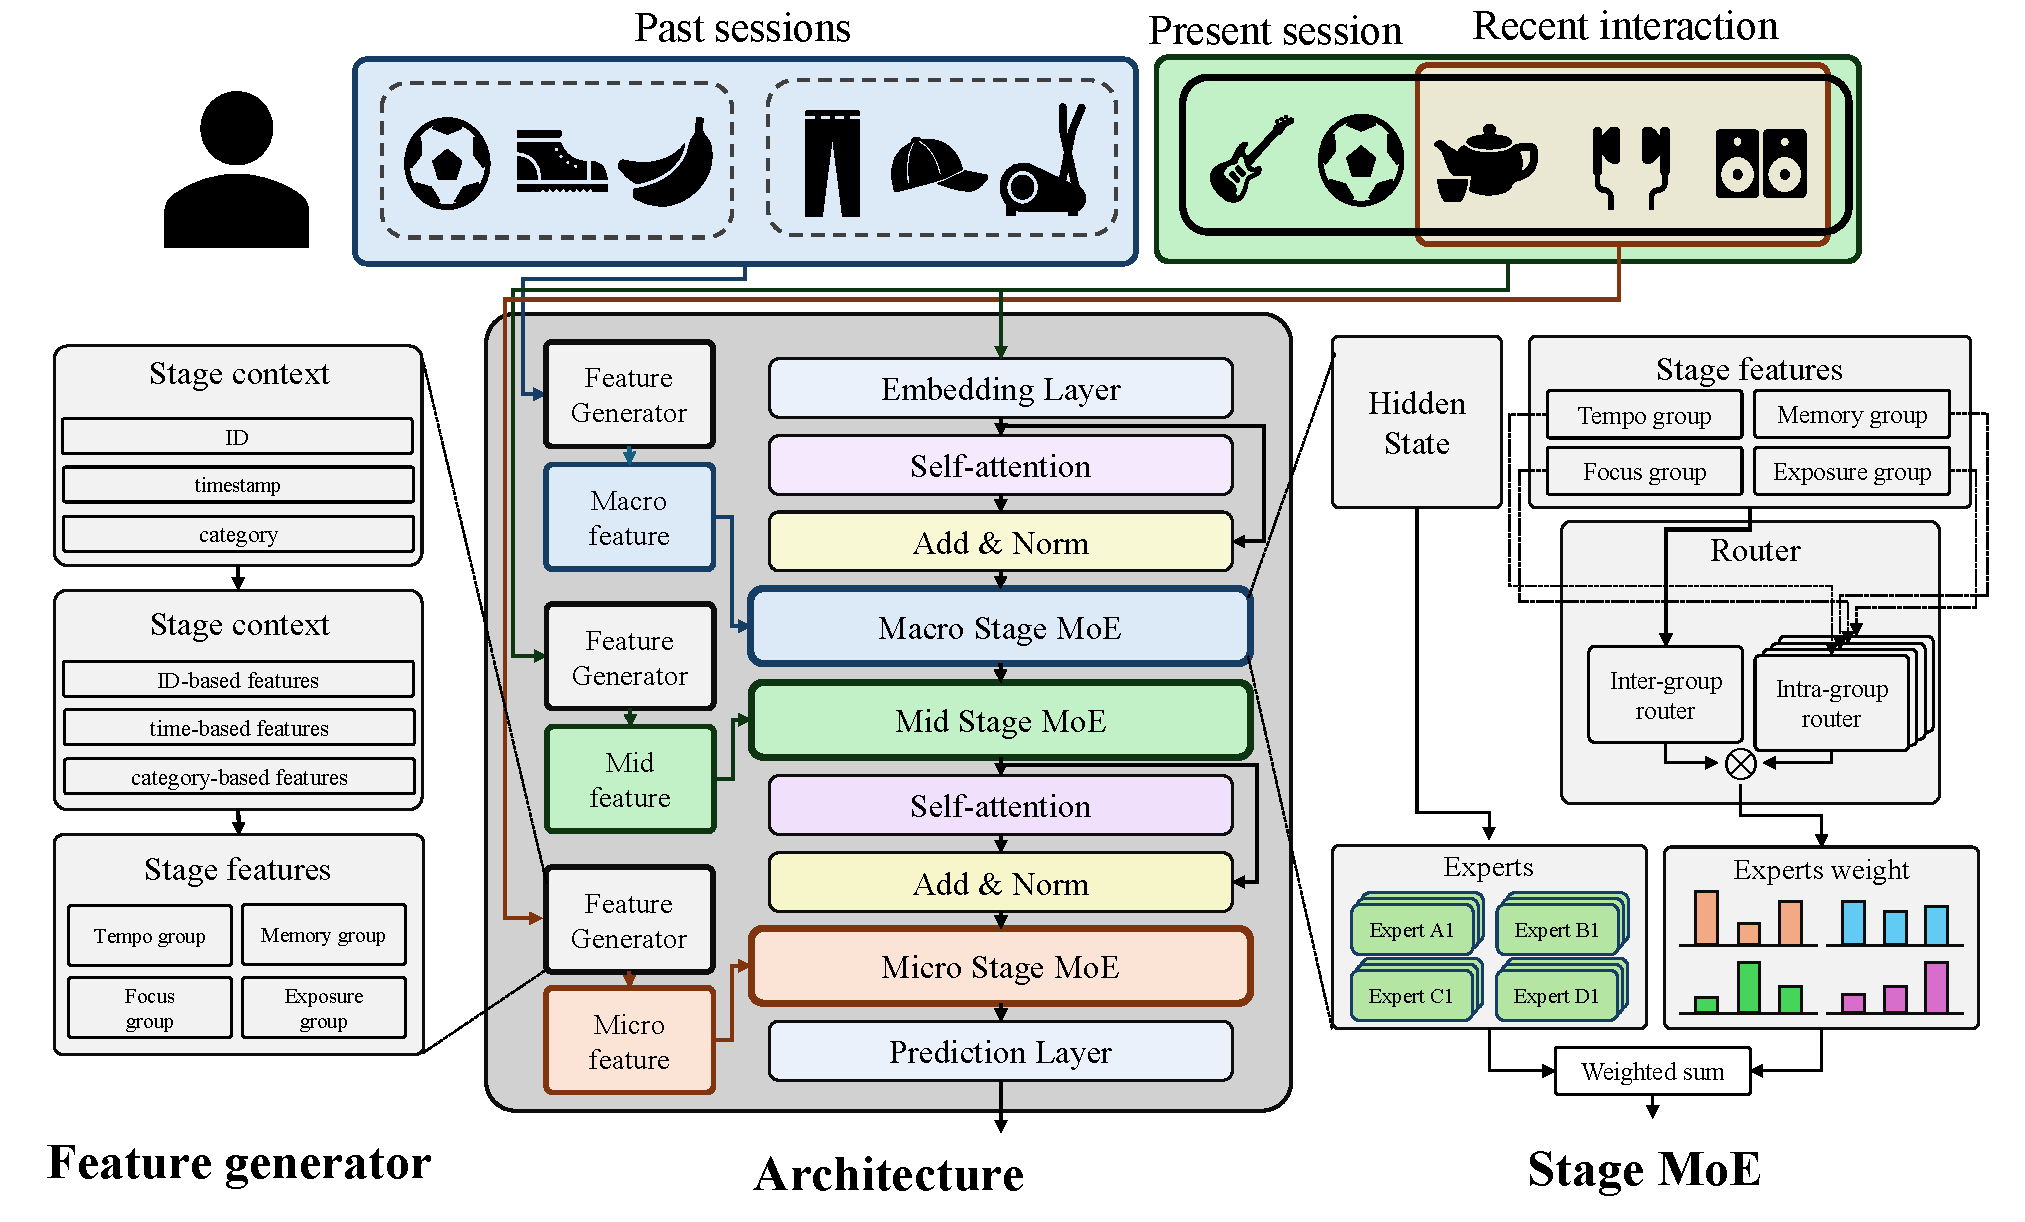
\includegraphics[width=0.95\textwidth]{figures/figure2_overall_arch_simple.pdf}
  \caption{Overall RouteRec framework. (a) RouteRec keeps a strong sequential backbone and replaces shared feed-forward blocks with behavior-guided sparse routing stages. (b) All stages use the same hierarchical sparse routing principle: group-level scores select a subset of semantic groups, then conditional intra-group scores select a subset of experts inside each chosen group before forming the active expert mixture. (c) Macro, mid, and micro differ by temporal evidence scope and routing granularity, not by the basic sparse routing logic. This figure is a framework-level view; the exact serial paper instantiation is specified in Method Section 3.3 and Appendix~\ref{app:method-details}.}
  \Description{A three-panel architecture figure showing RouteRec with a unified hierarchical sparse router across macro, mid, and micro stages, where stages differ by temporal evidence scope and granularity.}
  \label{fig:framework}
\end{figure*}

\section{Method}
\label{sec:method}

\subsection{RouteRec Overview}
\label{sec:problem-framework}

Figure~\ref{fig:framework} summarizes RouteRec at the framework level. For each user, we observe interactions ordered by time and train the model for next-item prediction. In one training instance, the observed prefix is denoted by $x_{1:t}$ and the target by $x_{t+1}$. Each interaction contains at least an item identity and timestamp, and may additionally include coarse category information depending on the dataset. RouteRec retains a strong sequential backbone for encoding the prefix, but replaces shared feed-forward computation with stage-wise sparse routing.

We first describe RouteRec as a design framework and refer to the fixed paper instantiation only when implementation choices matter. The model uses two signal channels: a representation channel that maps the prefix to hidden states transformed by experts, and a behavior channel that summarizes the same prefix into compact cues derived from ordinary logs. These cues are deliberately compact: they are routing controls, not another deep side branch. Broader variants are deferred to the appendix.

This design directly follows the challenge structure introduced earlier. Challenge~1 motivates portable behavior cues derived from widely available logs. Challenge~2 motivates stage-wise routing over macro, mid, and micro temporal scopes. Challenge~3 motivates decoupling behavior-grounded routing from the expert transformation pathway so that expert allocation can be analyzed in terms of observable behavior. The final paper instantiation adds sparse hierarchical activation at every stage, so that only a small subset of behavior-relevant expert groups and experts participates in each transformation. The remainder of this section formalizes how these ideas are instantiated in one RouteRec architecture.

Let $\mathcal{T}=\{\mathrm{macro},\mathrm{mid},\mathrm{micro}\}$ be the stage set. Let $\mathbf{h}^{\mathrm{in},(s)}_t$ denote the hidden state entering stage $s$. At stage $s \in \mathcal{T}$, routing uses a stage-specific behavior feature $\mathbf{f}^{(s)}_t$, while experts consume the current stage input state:
\begin{align}
\boldsymbol{\pi}^{(s)}_t
&=
\mathrm{softmax}\!\left(\mathrm{Router}_s(\mathbf{f}^{(s)}_t)/\tau_s\right), \\
\tilde{\mathbf{h}}^{(s)}_t
&=
\sum_{e=1}^{E}\pi^{(s)}_{t,e}\,\mathrm{Expert}^{(s)}_e(\mathbf{h}^{\mathrm{in},(s)}_t).
\label{eq:stage-routing}
\end{align}
Eq.~\eqref{eq:stage-routing} is the common stage interface. In the serial RouteRec architecture, each stage consumes the hidden state produced by the previous attention or routing block. Thus, the framework keeps one shared conditional-computation interface, while the paper instantiation specifies how these stage-local states are connected in sequence and sparsified.

\subsection{Portable Behavioral Cues}
\label{sec:feature-construction}

RouteRec is designed for realistic data availability. It uses signals commonly present in interaction logs: item identity, timestamp, optional coarse item-group labels, and corpus-level popularity statistics. We intentionally avoid heavy side-information encoders in the routing branch and instead use compact scalar summaries that remain easy to compute and inspect.

For session $s_m$ and target position $t$, the stage windows are
\begin{align}
\mathcal{R}^{\mathrm{macro}}_t &= [s_{\max(1,m-H)},\dots,s_{m-1}], \\
\mathcal{R}^{\mathrm{mid}}_t &= [x_1,\dots,x_{t-1}], \\
\mathcal{R}^{\mathrm{micro}}_t &= [x_{\max(1,t-w)},\dots,x_{t-1}],
\end{align}
where $H=5$ and $w=5$ in our main setting. These are the default paper windows used throughout the main experiments, and their role is revisited in the structural ablations in Appendix~\ref{app:stage-layout}. A shared summary operator $\mathcal{A}(\cdot)$ maps each window to a low-dimensional feature vector:
\[
\mathbf{f}^{(s)}_t=\mathcal{A}(\mathcal{R}^{(s)}_t),\qquad s\in\mathcal{T}.
\]

The summary dimensions are grouped into four semantic families: \textit{Tempo}, \textit{Focus}, \textit{Memory}, and \textit{Exposure}. Tempo captures coverage, pace, and interval dynamics. Focus captures concentration and switching behavior over the coarsest item-group proxy available in the dataset, such as product category, venue category, artist grouping, or genre. Memory captures repetition, overlap, and recurrence structure. Exposure captures the level, spread, and drift of interacted popularity. In the fixed paper instantiation, this family template yields a compact 16-dimensional cue bank per stage. When such grouping fields are unavailable, the corresponding focus cues are handled by the fixed missing-signal rule documented in Appendix~\ref{app:method-details}. Representative examples are listed in Table~\ref{tab:appendix-feature-families}.

The template is shared across stages, but each stage reads it through a different temporal lens: macro reflects persistent tendency, mid tracks evolving within-session intent, and micro emphasizes short-horizon cues near the prediction target. The goal is not to maximize handcrafted statistics, but to keep a small semantically legible cue bank that serves as a stable routing interface across datasets. Appendix~\ref{app:method-details} records the representative cue definitions and fixed paper setting.

\subsection{Coarse-to-Fine Multi-Stage Routing}

Although the router formula is shared, stages are not redundant. They differ in temporal evidence, routing granularity, and placement inside the backbone. In the fixed paper instantiation, the serial layout is
\[
\underbrace{\text{self-attn}}_{\text{context}} \to \text{macro} \to \text{mid} \to \underbrace{\text{self-attn}}_{\text{refresh}} \to \text{micro}.
\]
Let $\mathbf{h}^{(0)}_t$ denote the hidden state after the first attention block, $\mathbf{h}^{(1)}_t$ after macro routing, $\mathbf{h}^{(2)}_t$ after mid routing, and $\mathbf{h}^{(3)}_t$ after the second attention block. Macro, mid, and micro therefore consume $\mathbf{h}^{(0)}_t$, $\mathbf{h}^{(1)}_t$, and $\mathbf{h}^{(3)}_t$, respectively. The first attention layer contextualizes the prefix before routing. Macro and mid then provide slower sequence-level control over related contextual states, whereas the second attention layer is placed immediately before micro so that the final local router sees a refreshed token interaction state. Appendix~\ref{app:stage-layout} reports the broader layout ablations.

\paragraph{Macro and mid (sequence-wise routing).}
Macro and mid compute one routing distribution per sequence from their respective windows, then broadcast it over valid positions inside the sequence. Macro uses broader cross-session history; mid uses within-session prefix evidence. This setting emphasizes stable allocation for slower-changing context, where token-wise routing tended to add variance without introducing an equally meaningful control resolution in our ablations.

\paragraph{Micro (position-wise routing).}
Micro computes routing per token near the prediction target using short-horizon context. This enables fast adaptation to immediate transitions without changing the router form itself.

Formally, let $\bar{\mathbf{f}}_i^{\,(s)}$ denote the sequence-level cue summary used for sequence-wise routing at stage $s$. Then macro and mid use
\[
\begin{aligned}
\bar{\boldsymbol{\pi}}_i^{\,(s)}
&=
\mathrm{softmax}\!\left(\mathrm{Router}_s(\bar{\mathbf{f}}_i^{\,(s)})/\tau_s\right),
\qquad s\in\{\mathrm{macro},\mathrm{mid}\}, \\
\boldsymbol{\pi}^{(s)}_{i,t}
&=
\bar{\boldsymbol{\pi}}_i^{\,(s)}.
\end{aligned}
\]
Micro instead applies the same router form directly to position-specific cues,
\[
\boldsymbol{\pi}^{(\mathrm{micro})}_{i,t}
=
\mathrm{softmax}\!\left(\mathrm{Router}_{\mathrm{micro}}(\mathbf{f}^{(\mathrm{micro})}_{i,t})/\tau_{\mathrm{micro}}\right).
\]
Hence, RouteRec's coarse-to-fine behavior comes from stage evidence scope and update frequency, while the underlying router composition remains constant. The stages are therefore not repeated copies of the same router; they correspond to different temporal horizons at which behavioral evidence becomes informative for computation allocation. Because each stage captures a distinct control view, the final model uses sparse route commitment so that only a small subset of stage-relevant groups and experts is activated at each decision.

\subsection{Behavior-Guided Sparse Expert Allocation}

The final RouteRec architecture uses one shared hierarchical sparse composition at every stage. Experts are partitioned into $G$ groups with $C$ experts per group, so $E=GC$. For stage $s$ and position $t$, the router produces
\begin{align}
p^{(s)}_{t,g} &= \mathrm{softmax}_g\!\left(z^{(s)}_{t,g}\right), \\
r^{(s)}_{t,g,c} &= \mathrm{softmax}_c\!\left(u^{(s)}_{t,g,c}\right),
\end{align}
where $p^{(s)}_{t,g}$ is a group-level routing distribution and $r^{(s)}_{t,g,c}$ is a conditional within-group routing distribution. The final expert probability is their product:
\begin{equation}
\pi^{(s)}_{t,g,c}=p^{(s)}_{t,g}\,r^{(s)}_{t,g,c},
\label{eq:group-conditional-product}
\end{equation}
followed by flattening $(g,c)$ to expert index $e$. Eq.~\eqref{eq:group-conditional-product} is the same for macro, mid, and micro at the score level.

In the paper instantiation, groups are aligned with the four cue families, while multiple experts expand capacity within each group. This is a router-level semantic prior rather than a hard hand assignment of individual cues to experts. All three stages use the same feature-driven group-conditional router: a group-level router selects the relevant semantic control view, and a within-group router allocates capacity inside that view.

The final paper configuration adopts sparse activation at both routing levels. Let $\mathcal{K}^{(s)}_{t,\mathrm{grp}}$ be the index set of the top-$k_g$ groups under $p^{(s)}_{t,g}$ and $\mathcal{K}^{(s)}_{t,g,\mathrm{exp}}$ the index set of the top-$k_e$ experts under $r^{(s)}_{t,g,c}$ within group $g$. We then define the masked route
\begin{equation}
\hat{\pi}^{(s)}_{t,g,c}
=
\frac{\pi^{(s)}_{t,g,c}\,\mathbf{1}[g\in \mathcal{K}^{(s)}_{t,\mathrm{grp}}] \,\mathbf{1}[c\in \mathcal{K}^{(s)}_{t,g,\mathrm{exp}}]}{\sum_{g',c'} \pi^{(s)}_{t,g',c'}\,\mathbf{1}[g'\in \mathcal{K}^{(s)}_{t,\mathrm{grp}}] \,\mathbf{1}[c'\in \mathcal{K}^{(s)}_{t,g',\mathrm{exp}}]},
\label{eq:sparse-route}
\end{equation}
and use only the active experts in the stage transform:
\begin{equation}
\tilde{\mathbf{h}}^{(s)}_t
=
\sum_{g=1}^{G}\sum_{c=1}^{C}\hat{\pi}^{(s)}_{t,g,c}\,\mathrm{Expert}^{(s)}_{g,c}(\mathbf{h}^{\mathrm{in},(s)}_t).
\label{eq:sparse-stage-routing}
\end{equation}
In the selected paper setting, $G=4$ cue-aligned groups and $C=3$ experts per group. We choose $k_g=3$ and $k_e=2$, so each routing decision activates $3\times 2=6$ experts out of $12$ total experts. The semantic group prior therefore remains soft at the score level, but the executed computation path is explicitly sparse.

Sparse routing is introduced not only to reduce computation but also to enforce route commitment and sharpen specialization around a small active set. The hierarchical factorization keeps that selection interpretable by organizing it around semantic control views, while the experts themselves remain fully learned. Dense soft mixing is treated as an ablation variant rather than the final choice.

\subsection{Training Objective}
\label{sec:training-objective}

RouteRec is trained with a standard next-item objective and two router-side regularizers in the main paper configuration: route consistency and z-loss.

Let $\mathbf{z}$ be final logits and $y$ be the target item. The main loss is
\[
\mathcal{L}_{\mathrm{CE}}
=
-\log \frac{\exp z_y}{\sum_{j}\exp z_j}.
\]
For route consistency, we first compute a sample-level routing distribution at each stage by averaging token-level routing weights:
\[
\bar{\boldsymbol{\pi}}_i^{\,s}
=
\frac{1}{L_i}\sum_{t=1}^{L_i}\boldsymbol{\pi}_{i,t}^{\,s}
\]
where $L_i$ is the valid sequence length. We also form a stage-level cue summary
\[
\bar{\mathbf{f}}_i^{\,s}
=
\frac{1}{L_i}\sum_{t=1}^{L_i}\mathbf{f}_{i,t}^{\,s}.
\]
For each stage $s$, we construct a pair set $\mathcal{P}_s$ from the $k_{\mathrm{nn}}$ nearest non-self samples in the mini-batch according to cosine similarity between these stage-level cue summaries, and minimize
\[
\mathcal{L}_{\mathrm{cons}}
=
\frac{1}{|\mathcal{T}|}
\sum_{s \in \mathcal{T}}
\frac{1}{|\mathcal{P}_s|}
\sum_{(i,j)\in \mathcal{P}_s}
\mathrm{JSD}\!\left(\bar{\boldsymbol{\pi}}_i^{\,s}, \bar{\boldsymbol{\pi}}_j^{\,s}\right),
\]
which encourages neighboring behavioral states to produce compatible routing distributions. Appendix~\ref{app:method-details} reports the neighbor setting used in the paper instantiation.
To stabilize gating numerics, we adopt z-loss on the pre-softmax expert logits $a_{i,t,e}^{\,s}$~\cite{zoph2022stmoe}:
\[
\mathcal{L}_{z}
=
\frac{1}{|\mathcal{T}|}
\sum_{s \in \mathcal{T}}
\frac{1}{N_s}
\sum_{(i,t)\in\mathcal{V}_s}
\left(
\log \sum_{e=1}^{E}\exp a_{i,t,e}^{\,s}
\right)^2,
\]
where $\mathcal{V}_s$ is the set of valid positions and $N_s=|\mathcal{V}_s|$. The final objective is
\[
\mathcal{L}
=
\mathcal{L}_{\mathrm{CE}}
+
\lambda_{\mathrm{cons}}\,\mathcal{L}_{\mathrm{cons}}
+
\lambda_{z}\,\mathcal{L}_{z},
\]
where $\lambda_{\mathrm{cons}}$ and $\lambda_z$ are trade-off coefficients. Unlike classical MoE setups that explicitly enforce uniform expert traffic, the selected main configuration does not include load balancing. The aim is stable, behavior-aligned specialization rather than equal usage for its own sake. Appendix~\ref{app:objective} reports the objective variants.

\section{Experiments}
\label{sec:experiments}


\subsection{Experimental Setup}
We evaluate RouteRec on six public datasets spanning e-commerce, POI recommendation, short-video consumption, music listening, movie preference, and anonymous clickstream behavior: Beauty, Foursquare, KuaiRec, LastFM, ML-1M, and Retail Rocket. Appendix~B summarizes their provenance and processed statistics.

\begin{table*}[!b]
  \caption{Seen-target test results under the sessionized temporal protocol. Datasets marked with $^\dagger$ are sampled processed subsets (KuaiRec 20\%, LastFM 3\%). For each method, we report the seen-target test metrics of the run achieving the highest mean seen-target test score over the nine reported metrics. Avg.~Rank is computed over all rows in this table, where lower is better. The RouteRec column is shaded for readability.}
  \label{tab:main-overall}
  \centering
  \small
  \setlength{\tabcolsep}{3.4pt}
  \renewcommand{\arraystretch}{1.05}
  \resizebox{\textwidth}{!}{%
  \begin{tabular}{ll*{9}{c}>{\columncolor{routerecgray}}c}
    \toprule
    Dataset & Metric & SASRec & GRU4Rec & TiSASRec & FEARec & DuoRec & BSARec & FAME & DIF-SR & FDSA & RouteRec \\
    \midrule
    \multirow{3}{*}{Beauty}
      & HR@10   & 0.1279 & 0.0774 & \tblbest{0.1579} & 0.0229 & 0.1433 & 0.0372 & 0.0372 & 0.0258 & 0.1433 & \tblsecond{0.1490} \\
      & NDCG@10 & 0.0770 & 0.0433 & \tblbest{0.1015} & 0.0167 & 0.0823 & 0.0187 & 0.0239 & 0.0157 & \tblsecond{0.0955} & 0.0922 \\
      & MRR@20  & 0.0639 & 0.0349 & \tblbest{0.0873} & 0.0154 & 0.0675 & 0.0137 & 0.0214 & 0.0130 & \tblsecond{0.0828} & 0.0790 \\
    \midrule
    \multirow{3}{*}{Retail Rocket}
      & HR@10   & 0.5327 & 0.4943 & 0.5248 & \tblbest{0.5620} & 0.5548 & 0.5117 & 0.4694 & 0.4811 & 0.5484 & \tblsecond{0.5609} \\
      & NDCG@10 & 0.3913 & 0.3548 & 0.3780 & \tblbest{0.4168} & 0.4070 & 0.4022 & 0.4000 & 0.4058 & 0.4036 & \tblsecond{0.4152} \\
      & MRR@20  & 0.3513 & 0.3158 & 0.3362 & 0.3757 & 0.3654 & 0.3707 & \tblsecond{0.3787} & \tblbest{0.3830} & 0.3627 & 0.3742 \\
    \midrule
    \multirow{3}{*}{Foursquare}
      & HR@10   & 0.3102 & 0.2190 & 0.2996 & 0.3054 & \tblsecond{0.3137} & 0.2610 & 0.2358 & 0.2554 & 0.3054 & \tblbest{0.3221} \\
      & NDCG@10 & 0.1935 & 0.1476 & 0.1895 & 0.1906 & 0.2005 & 0.1735 & 0.1598 & 0.1738 & \tblsecond{0.2026} & \tblbest{0.2059} \\
      & MRR@20  & 0.1609 & 0.1284 & 0.1586 & 0.1589 & 0.1699 & 0.1489 & 0.1385 & 0.1506 & \tblbest{0.1736} & \tblbest{0.1736} \\
    \midrule
    \multirow{3}{*}{ML-1M}
      & HR@10   & 0.1474 & 0.1468 & 0.1563 & 0.1310 & 0.1557 & 0.1515 & \tblbest{0.1645} & 0.1520 & \tblsecond{0.1599} & 0.1543 \\
      & NDCG@10 & 0.0726 & 0.0762 & 0.0834 & 0.0632 & 0.0774 & 0.0818 & \tblbest{0.0867} & 0.0806 & \tblsecond{0.0848} & 0.0819 \\
      & MRR@20  & 0.0556 & 0.0594 & 0.0666 & 0.0476 & 0.0589 & 0.0651 & \tblbest{0.0678} & 0.0643 & \tblsecond{0.0670} & 0.0655 \\
    \midrule
    \multirow{3}{*}{LastFM$^\dagger$}
      & HR@10   & 0.3712 & 0.3097 & 0.3577 & \tblsecond{0.3867} & 0.3853 & 0.3395 & 0.3399 & 0.3686 & 0.3769 & \tblbest{0.3958} \\
      & NDCG@10 & 0.3078 & 0.2616 & 0.3041 & 0.3240 & 0.3186 & 0.2996 & 0.2979 & 0.3199 & \tblsecond{0.3260} & \tblbest{0.3326} \\
      & MRR@20  & 0.2893 & 0.2484 & 0.2891 & 0.3053 & 0.2989 & 0.2879 & 0.2856 & 0.3061 & \tblsecond{0.3120} & \tblbest{0.3141} \\
    \midrule
    \multirow{3}{*}{KuaiRec$^\dagger$}
      & HR@10   & 0.3404 & 0.3035 & 0.3277 & \tblsecond{0.3606} & 0.3572 & 0.3371 & 0.3348 & 0.3247 & 0.3449 & \tblbest{0.3718} \\
      & NDCG@10 & 0.3179 & 0.2520 & 0.3092 & 0.3325 & 0.3297 & \tblsecond{0.3342} & 0.3326 & 0.3163 & 0.3158 & \tblbest{0.3479} \\
      & MRR@20  & 0.3120 & 0.2379 & 0.3049 & 0.3259 & 0.3229 & \tblsecond{0.3335} & 0.3320 & 0.3148 & 0.3083 & \tblbest{0.3423} \\
    \midrule
    \multicolumn{2}{l}{\textbf{Avg.~Rank$\downarrow$}} & \textbf{6.00} & \textbf{8.89} & \textbf{5.61} & \textbf{5.31} & \textbf{4.25} & \textbf{6.53} & \textbf{6.08} & \textbf{6.56} & \textbf{3.61} & \textbf{2.17} \\
    \bottomrule
  \end{tabular}}
\end{table*}

Across datasets, we use a sessionized temporal protocol assembled from established session-based and session-aware practice rather than a canonical raw-sequence leaderboard setting~\cite{jannach2022sessions,quadrana2017hrnn,latifi2021sessionaware}. Interactions are ordered chronologically, sessionized with inactivity heuristics, and iteratively filtered to remove sessions shorter than $5$ and items with fewer than $3$ interactions~\cite{li2017narm,wu2019srgnn}. We use a 30-minute threshold for Foursquare, KuaiRec, LastFM, ML-1M, and Retail Rocket, and a 14-day threshold for the much sparser Beauty review stream~\cite{quadrana2017hrnn,lacic2020jobsessions,borgbruun2022insurance}. KuaiRec and LastFM are reported on processed sampled subsets (20\% and 3\%, respectively). After preprocessing, sessions are sorted by start time and split chronologically into 70\%/15\%/15\% train/validation/test partitions. Appendix~B gives the full preprocessing and held-out cleanup details~\cite{ji2023leakage,gusak2025timesplit}.

Our main comparison uses the seen-target view, since ID-based recommenders cannot rank items absent from the training vocabulary and session-aware benchmarks typically treat unseen targets as supplementary accounting rather than the primary comparison~\cite{latifi2021sessionaware,li2017narm,wu2019srgnn}. We compare against GRU4Rec, SASRec, TiSASRec, DuoRec, FEARec, BSARec, FAME, DIF-SR, and FDSA~\cite{hidasi2016gru4rec,kang2018sasrec,li2020tisasrec,qiu2022duorec,du2023fearec,shin2024bsarec,liu2025fame,xie2022difsr,zhang2019fdsa}. All methods use the same processed files, the same optimization family, matched early stopping, and the same model-selection rule.

We treat tuning as part of the protocol rather than as a secondary implementation detail. Each model is searched within a fixed bounded grid of shared optimization hyperparameters plus a small number of model-specific controls, and any adaptive search remains restricted to those predeclared candidate sets and the same validation files and stopping rule for all methods~\cite{galuzzi2020bayesopt}. RouteRec uses no extra held-out sessions or external metadata at evaluation time; its routing cues are deterministic summaries of the same observed histories used by every method. Appendix~B reports the exact grids, budgets, processed statistics, and full $k\in\{5,10,20\}$ tables.

The main experimental section is organized around five questions: \textbf{Q1)} ranking quality, \textbf{Q2)} routing control, \textbf{Q3)} design justification, \textbf{Q4)} practicality, and \textbf{Q5)} routing semantics. Reduced-cue portability studies and broader structural sweeps are deferred to the appendix.

This organization is deliberate for the paper narrative. Q1 establishes whether behavior-guided routing is worth considering at all under a shared sessionized protocol, Q2 and Q3 test whether the gain is actually tied to routing control and staged structure, Q4 checks whether that design remains practical once sparsity is enforced, and Q5 returns to the original semantic claim by asking whether the learned routes vary in the way the method intends.

\begin{figure*}[!t]
  \centering
  \begin{minipage}[t]{0.438\textwidth}
    \centering
    
\includegraphics[width=\linewidth]{figures/fig_q2_routing_control_a.pdf}
    \vspace{0.1em}
    {\footnotesize (a) Dynamic-dataset group: same five controls}
  \end{minipage}\hfill
  \begin{minipage}[t]{0.438\textwidth}
    \centering
    
\includegraphics[width=\linewidth]{figures/fig_q2_routing_control_b.pdf}
    \vspace{0.1em}
    {\footnotesize (b) Stable/mixed-dataset group: same five controls}
  \end{minipage}
  \caption{Routing-control comparison across two dataset groups. Both panels use the same five variants and differ only in dataset grouping, isolating how the routing-control choice behaves in dynamic versus more stable settings.}
  \Description{Two panels comparing the same five routing-control variants across dynamic and stable/mixed dataset groups.}
  \label{fig:routing-control-panels}
\end{figure*}

\subsection{Q1. Does RouteRec Improve Ranking Quality?}
\label{sec:overall-performance}
Table~\ref{tab:main-overall} presents the main seen-target comparison in the text using HR@10, NDCG@10, and MRR@20, together with an Avg.~Rank summary across all reported rows. This presentation keeps the main paper focused on a compact set of representative cutoffs, while Appendix~B reports the full $k\in\{5,10,20\}$ grid under the same selection rule. Under this view, RouteRec delivers the strongest overall rank, leads on Foursquare, LastFM, and the sampled KuaiRec subset, remains close to the top on Beauty and Retail Rocket, and stays competitive on ML-1M even when the strongest baseline there remains slightly ahead.

The baseline pattern is also informative. SASRec and TiSASRec remain consistently strong under this protocol, which is plausible because the sessionized split produces relatively short, recency-sensitive prefixes where strong autoregressive self-attention and explicit interval modeling already capture much of the available signal~\cite{kang2018sasrec,li2020tisasrec}. By contrast, BSARec is less competitive here even though it is strong in standard longer-sequence settings: its attentive frequency bias is designed to exploit richer global spectral structure~\cite{shin2024bsarec}, and that advantage is naturally attenuated when sessionization shortens contexts and reduces long-range periodic evidence. DIF-SR also improves less in this setup, which is consistent with its side-information-fusion focus~\cite{xie2022difsr}: under our shared protocol, auxiliary features are intentionally lightweight and heterogeneous across datasets, so the side branch contributes less additional structure than in richer feature regimes. These gaps should therefore be read as protocol- and inductive-bias-dependent behavior rather than as evidence of under-tuning, since all methods follow the same bounded search, stopping rule, and processed files.

Overall, Q1 shows that RouteRec is competitive under the shared sessionized protocol, with the clearest gains in the more behaviorally dynamic settings.

\subsection{Q2. What Should Control Routing?}
\label{sec:routing-control}
Figure~\ref{fig:routing-control-panels} compares five variants that separate where behavior information is used: a shared FFN, hidden-only routing, feature fusion by additive bias, mixed hidden+behavior routing, and the final behavior-guided sparse router. Hidden-only routing can improve over a shared FFN, and simple feature reinjection is not entirely ineffective, but neither yields the same consistency as using behavior cues directly as routing controls. The final behavior-guided design therefore outperforms representation-only feature injection and avoids collapsing the routing signal back into hidden-state geometry.

Both panels use the same five variants and differ only in dataset grouping. Panel (a) emphasizes more behaviorally dynamic datasets, whereas Panel (b) reports the more stable or mixed group. Appendix~\ref{app:objective} reports the corresponding objective variants separately so that the routing-signal effect is not conflated with the loss choice.

The practical takeaway is that the best routing signal is not the one that carries the most raw information, but the one that exposes the cleanest control boundary. Once behavior cues are used directly at the router, RouteRec can let the representation path focus on sequence modeling while the router absorbs cross-dataset differences in pace, focus, and recurrence more explicitly.

\begin{figure*}[!t]
  \centering
  \begin{minipage}[t]{0.438\textwidth}
    \centering
    
\includegraphics[width=\linewidth]{figures/fig_q3_design_justification_a.pdf}
    \vspace{0.1em}
    {\footnotesize (a) Temporal decomposition matters}
  \end{minipage}\hfill
  \begin{minipage}[t]{0.438\textwidth}
    \centering
    
\includegraphics[width=\linewidth]{figures/fig_q3_design_justification_b.pdf}
    \vspace{0.1em}
    {\footnotesize (b) Hierarchical sparse routing matters}
  \end{minipage}
  \caption{Design-justification ablations. Panel (a) compares the final three-stage design against reduced temporal decompositions, and Panel (b) compares flat versus hierarchical and dense versus sparse routing organizations.}
  \Description{Two panels for RouteRec's design justification: temporal decomposition and routing organization.}
  \label{fig:stage-structure-panels}
\end{figure*}

\subsection{Q3. Why Is RouteRec's Three-Part Design Effective?}
\label{sec:stage-structure}
Figure~\ref{fig:stage-structure-panels} tests whether RouteRec's gains come from the three-part design itself rather than from expert insertion alone. Panel (a) asks whether temporal decomposition is necessary by comparing the final three-stage design against the best reduced single-view and two-view alternatives. Panel (b) asks whether the selected routing organization is meaningful by comparing flat versus hierarchical routing and sparse versus dense allocation under comparable expert pools.

Taken together, these ablations test whether RouteRec's gain comes from temporal decomposition and hierarchical sparse commitment rather than indiscriminate expert insertion. Broader scope-order and portability controls are deferred to the appendix.

The pattern is consistent with the method hypothesis. A single behavior view is too coarse to separate slow tendency from immediate transition pressure, while a dense flat expert pool weakens route commitment even when the total expert budget is comparable. The selected three-stage sparse hierarchy is therefore useful because it assigns different temporal questions to different routing decisions instead of asking one router to absorb all scopes at once.

\subsection{Q4. Is RouteRec Practical as a Sparse Design?}
\label{sec:efficiency}
Q4 asks whether the final sparse RouteRec design remains practical in cost. On two representative datasets, sparse RouteRec uses 3.2M total parameters but only 1.6M active parameters per routed decision, compared with 3.2M active parameters for the dense variant and 1.8M for SASRec. Its train and inference ratios are $1.42\times$ and $1.18\times$ relative to SASRec, versus $1.85\times$ and $1.38\times$ for dense RouteRec. The key distinction is therefore executed capacity rather than total capacity alone. Appendix~\ref{app:efficiency} reports the full efficiency summary.

This gap matters for the paper claim because it shows that RouteRec is not simply buying accuracy through unrestricted dense over-parameterization. The sparse design still pays a modest routing overhead, but it keeps the active compute budget much closer to strong shared-path baselines than the dense expertized alternative does.

\subsection{Q5. What Does the Learned Router Actually Capture?}
\label{sec:behavior-regimes}
Figure~\ref{fig:behavior-regime-panels} addresses the most direct semantic question raised by the method: if RouteRec is designed to react to behavioral regimes, then representative repeat-heavy, fast exploratory, and narrow-focus cases should exhibit different stage-wise routing maps. We therefore present three representative routing cases in the main text and retain intervention-based perturbation results as supporting evidence for the appendix and discussion.

\begin{figure*}[!t]
  \centering
  \begin{minipage}[t]{0.292\textwidth}
    \centering
    
\includegraphics[width=\linewidth]{figures/appendix/a05_routing_profiles_a.pdf}
  \end{minipage}\hfill
  \begin{minipage}[t]{0.292\textwidth}
    \centering
    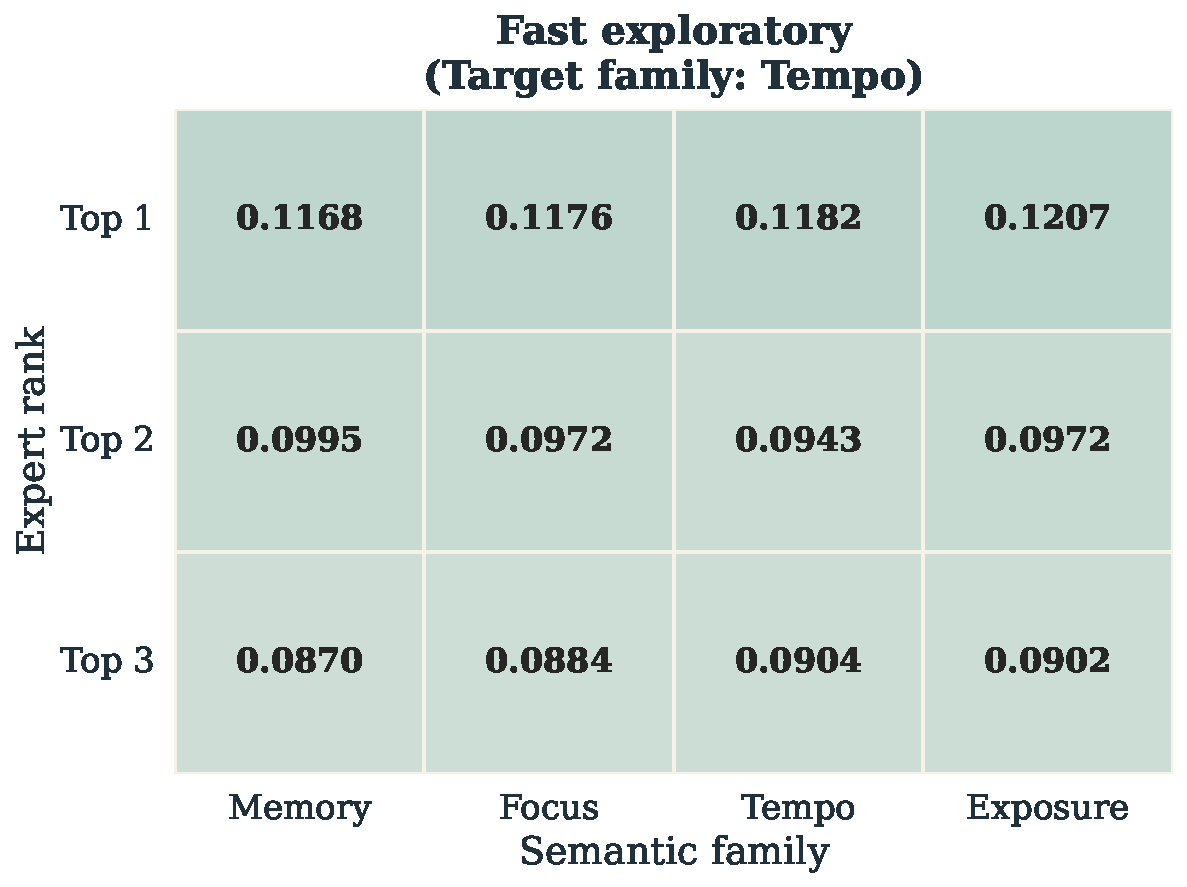
\includegraphics[width=\linewidth]{figures/appendix/a05_routing_profiles_b.pdf}
  \end{minipage}\hfill
  \begin{minipage}[t]{0.292\textwidth}
    \centering
    
\includegraphics[width=\linewidth]{figures/appendix/a05_routing_profiles_c.pdf}
  \end{minipage}
  \caption{Representative routing semantics. Cases are defined by simple post hoc statistics: repeat-heavy, fast exploratory, and narrow-focus. Each panel shows how stage-wise semantic-group emphasis shifts across regimes.}
  \Description{Three-panel figure showing stage-aware routing maps for repeat-heavy, fast exploratory, and narrow-focus behavioral cases.}
  \label{fig:behavior-regime-panels}
\end{figure*}

This analysis connects the empirical evidence back to the motivation in Figure~\ref{fig:intro-behavioral-features}. To avoid circularity, the cases are selected from simple post hoc statistics derived from raw interaction histories rather than optimized labels or supervision targets. Appendix-level cue interventions support the same reading.

The three cases also clarify why the method is most compelling on dynamic datasets. When repeat structure, short-horizon tempo, or concentration shifts become more pronounced, the stage-local router has a clearer reason to deviate from a shared computation path. In more preference-stable settings, the same mechanism remains competitive but is asked to differentiate less sharply, which is consistent with the smaller margin observed on ML-1M.

Detailed full-cutoff results and extended analyses, including exact sparse-routing specification, reduced-cue portability studies, broader structural ablations, sparse-design controls, objective variants, extended efficiency summaries, routing diagnostics, intervention studies, and transfer experiments, are reported in Appendices~A--K.

\section{Conclusion}
\label{sec:conclusion}
RouteRec starts from a simple hypothesis: when behavioral evidence changes, the computation path should change as well. The experiments support that view from three angles. First, RouteRec improves next-item ranking most clearly on behaviorally dynamic datasets and remains competitive elsewhere, although the advantage narrows in more preference-stable settings such as ML-1M. Second, the gain is tied to the routing signal, staged temporal decomposition, and sparse route commitment rather than indiscriminate expert insertion. Third, compact cues derived from ordinary interaction logs preserve a meaningful share of the benefit, keeping the method practical when side information is limited.

Taken together, the results suggest that behavior-guided routing can be both semantically meaningful and computationally selective. In the selected paper setting, portable cues, coarse-to-fine routing, and behavior-guided sparse expert allocation form a compact interface for conditional computation. Future work can extend that interface through adaptive sparsity budgets, transfer of routing priors across domains, more robust cue construction, and tighter deployment-aware constraints.

More broadly, the paper suggests a useful modeling stance for sessionized recommendation: not every gain from extra capacity should be interpreted as better sequence representation. Some of it can come from exposing a better control interface over when different computations should be used at all. RouteRec's contribution is to make that interface explicit, lightweight, and inspectable.

\clearpage
\balance
\bibliographystyle{ACM-Reference-Format}
\bibliography{refs}

\clearpage
\appendix

\section{Exact RouteRec Instantiation and Sparse Routing Formulation}
\label{app:method-details}
This appendix records the fixed paper instantiation and the representative cue bank used by RouteRec. Whereas the main text emphasizes the conceptual design axes, this section documents the implementation choices that are relevant for reproducibility and for interpreting the later ablations, with the sparse routing formulation made explicit.

\subsection{Main Paper Configuration}

\begin{table}[H]
  \centering
  \caption{Fixed main configuration used in the paper.}
  \label{tab:appendix-main-setting}
  \footnotesize
  \setlength{\tabcolsep}{4pt}
  \renewcommand{\arraystretch}{1.07}
  \begin{tabularx}{\columnwidth}{@{}L{0.30\columnwidth}>{\raggedright\arraybackslash}X@{}}
    \toprule
    Aspect & Main paper configuration \\
    \midrule
    Backbone layout & self-attn $\to$ macro block $\to$ mid block $\to$ self-attn $\to$ micro block \\
    Stage execution & Serial \\
    Routing granularity & Macro and mid: sequence-wise; micro: position-wise \\
    Router composition & Shared hierarchical sparse router at all three stages \\
    Expert activation & Top-$3$ groups out of $4$; top-$2$ experts per selected group \\
    Active experts & $6$ out of $12$ total per routed decision \\
    History windows & $H=5$ sessions (macro); $w=5$ positions (micro) \\
    Core auxiliary terms & Route consistency + z-loss; no load balancing \\
    \bottomrule
  \end{tabularx}
\end{table}

The placement of the two attention layers reflects the intended temporal roles of the stages. The first attention layer contextualizes the raw prefix before any routing is applied. Macro and mid then operate consecutively because both provide slower sequence-level control over the same contextualized sequence state: macro captures broader recent-history tendency, while mid refines within-session evolution. A second attention layer is inserted only before micro so that the final local router receives a refreshed token interaction state immediately before prediction. This layout was the most stable high-performing architecture in our architecture sweep, and Appendix~\ref{app:stage-layout} compares it against denser and differently ordered alternatives.

This table serves as a reproducibility summary rather than as a search-space description. Architectural choices are fixed across the paper track, whereas capacity and optimization values are selected per dataset from a narrow candidate set and are therefore reported as compact ranges only when no single global value is shared across all reported runs.

\subsection{Implementation Specification and Minimal Execution Notes}

\begin{table}[H]
  \centering
  \caption{Implementation-level settings used in the selected paper track.}
  \label{tab:appendix-implementation-spec}
  \footnotesize
  \setlength{\tabcolsep}{4pt}
  \renewcommand{\arraystretch}{1.07}
  \begin{tabularx}{\columnwidth}{@{}L{0.30\columnwidth}>{\raggedright\arraybackslash}X@{}}
    \toprule
    Item & Reported setting \\
    \midrule
    Semantic groups & $G=4$ groups: Tempo, Focus, Memory, Exposure \\
    Experts per group & $C\in\{2,3,4\}$; total experts $E=4C$ \\
    Main sparse setting & $C=3$, top-$3$ groups, top-$2$ experts per selected group \\
    Cue dimensionality & $16$ scalars per stage \\
    Router hidden width & Representative range $48$--$128$ \\
    Routing temperature & Macro $1.0$; mid and micro $1.2$ \\
    Consistency neighbors & $k_{\mathrm{nn}}=1$ nearest non-self sample per stage \\
    Missing-signal handling & Broadcast when available; zero-fill focus cues if grouping field absent \\
    \bottomrule
  \end{tabularx}
\end{table}

\noindent\textbf{Minimal execution notes.}
The implementation uses three simple rules that are easy to miss if one only reads the high-level method description. First, macro and mid cues are computed once per example and then broadcast over the routed positions, whereas micro cues are evaluated at the position level. Second, top-$k$ masking is followed by re-normalization inside the active support rather than by leaving the logits in an unnormalized sparse state. Third, if a dataset does not expose the grouping field needed for focus-family cues, the implementation falls back to the fixed missing-signal policy in Table~\ref{tab:appendix-implementation-spec} rather than silently redefining the cue family per dataset.

\subsection{Representative Behavioral Cue Families}

\begin{table*}[!t]
  \centering
  \caption{Representative cue summaries used by RouteRec in the main configuration. Each stage uses four semantic families with four scalar summaries per family; the table lists representative examples rather than every implementation detail.}
  \label{tab:appendix-feature-families}
  \footnotesize
  \setlength{\tabcolsep}{4pt}
  \renewcommand{\arraystretch}{1.05}
  \begin{tabularx}{\textwidth}{@{}lXXX@{}}
    \toprule
    Family & Macro (recent-session tendency) & Mid (within-session evolution) & Micro (short-horizon pressure) \\
    \midrule
    Tempo & Context-valid ratio, last inter-session gap, mean pace, pace trend & Valid-prefix ratio, mean/std interaction interval, session age & Last gap, short-window mean gap, short-window std, deviation from mid-scale pace \\
    Focus & Theme entropy, dominant-theme mass, theme repeat rate, theme shift rate & Category entropy, category top-1 mass, category switch rate, category uniqueness & Immediate category switch, mismatch to recent category history, suffix entropy, suffix uniqueness \\
    Memory & Repeat intensity, adjacent category overlap, adjacent item overlap, repeat trend & Item uniqueness, repeat rate, novelty rate, longest item run & Reconsumption flag, suffix reconsumption rate, suffix item uniqueness, suffix longest run \\
    Exposure & Mean popularity, popularity spread, popularity entropy, popularity trend & Mean popularity, popularity std, popularity entropy, popularity drift & Last-item popularity, suffix popularity spread, suffix popularity entropy, deviation from mid-scale popularity \\
    \bottomrule
  \end{tabularx}
\end{table*}

This cue bank is intentionally compact. The feature families are hand-designed in the sense that they encode behavioral hypotheses, but the design goal is to keep them as a small set of summaries that can serve as a stable routing interface across datasets. In practice, the macro bank is instantiated from the recent-session window used by the selected paper instantiation, while mid and micro are computed from the current session prefix at different temporal scopes. The main text therefore reports the family structure and representative examples, while this appendix provides the implementation-oriented view.

\section{Dataset, Evaluation, and Full Ranking Results}

All experiments were conducted on machines equipped with NVIDIA RTX 3090 24\,GB GPUs. Each training or evaluation process used a single GPU; multiple GPUs were used only to run independent experiments in parallel, not for multi-GPU training within a single run.
\label{app:data-details}
This appendix summarizes the six datasets and makes the evaluation protocol explicit, since recent work has shown that session construction and split strategy can materially affect offline recommender results~\cite{ji2023leakage,gusak2025timesplit}. The original releases are cited here for completeness~\cite{mcauley2015amazon,yang2010foursquare,gao2022kuairec,celma2010music,harper2015movielens,retailrocket2015dataset}. The dataset descriptions emphasize domain differences and signal availability because the routing branch depends on which behavioral evidence is exposed in each corpus.

\subsection{Datasets and Protocol}

\begin{table}[H]
  \caption{Datasets used in the experiments. Datasets marked with $^\dagger$ are sampled processed subsets.}
  \label{tab:appendix-datasets}
  \centering
  \footnotesize
  \setlength{\tabcolsep}{3.0pt}
  \begin{tabular*}{\columnwidth}{@{\extracolsep{\fill}}llrrrc@{}}
    \toprule
    Dataset & Domain & Interactions & Sessions & Items & Avg. len. \\
    \midrule
    Beauty & E-com. & 33,488 & 4,243 & 3,625 & 7.9 \\
    Foursquare & POI & 145,238 & 25,369 & 30,588 & 5.7 \\
    KuaiRec$^\dagger$ & Video & 287,411 & 24,458 & 6,477 & 11.8 \\
    LastFM$^\dagger$ & Music & 470,408 & 25,089 & 52,510 & 18.8 \\
    ML-1M & Movie & 575,281 & 14,539 & 3,533 & 39.6 \\
    Retail Rocket & Browse & 821,243 & 153,092 & 90,211 & 5.4 \\
    \bottomrule
  \end{tabular*}
\end{table}

Table~\ref{tab:appendix-datasets} reports the statistics of the final processed datasets used in the experiments rather than the raw corpus sizes. In particular, KuaiRec corresponds to the 20\% processed subset used in our runs, and LastFM corresponds to the 3\% processed subset.

For reproducibility, the protocol is summarized as follows.
\begin{enumerate}
  \item Sort all interactions chronologically within each dataset.
  \item Reconstruct sessions with a dataset-specific inactivity threshold.
  \item Iteratively prune sessions with length below $5$ and items with support below $3$ until the constraints are simultaneously satisfied.
  \item Sort the resulting sessions by session start time.
  \item Assign the earliest 70\% of sessions to train and treat the latest 30\% as a held-out tail.
  \item Build validation and test from the held-out tail under chronology-preserving cleanup.
  \item Report seen-target metrics as the primary view and keep unseen-target behavior as supplementary accounting.
\end{enumerate}

Beauty and Retail Rocket stress sparse e-commerce revisit behavior, Foursquare and KuaiRec emphasize stronger short-horizon intent changes, and LastFM and ML-1M provide longer preference-driven histories. This spread makes it possible to examine whether behavior-guided routing is primarily beneficial in highly dynamic settings or remains competitive when preference structure is more stable.

Signal availability also differs in a way that matters for routing. Beauty exposes item, time, and product-category cues after low-rating removal. Foursquare includes item, timestamp, and venue-category structure with bursty check-in dynamics. KuaiRec offers item, time, and coarse content-side metadata in short-video sessions with strong short-term intent shifts. LastFM provides repeated listening histories with artist-side signals, while ML-1M contributes longer preference-driven sequences with genre information. Retail Rocket is the sparsest side-information setting, relying mainly on anonymous event streams with item and time signals.

We position our setup as a sessionized sequential evaluation protocol assembled from established components, not as the canonical raw-sequence protocol for sequential recommendation~\cite{jannach2022sessions,quadrana2017hrnn,latifi2021sessionaware}. Sessions are reconstructed post hoc with inactivity heuristics, which is standard practice when logs do not provide explicit session boundaries~\cite{jannach2022sessions}. The thresholds are adapted to the logging regime of each corpus: Foursquare, KuaiRec, LastFM, ML-1M, and Retail Rocket use a 30-minute inactivity threshold, consistent with dense-log session-aware practice~\cite{quadrana2017hrnn,lacic2020jobsessions}, whereas Beauty uses a 14-day threshold because review timestamps are substantially more diffuse. More generally, this threshold choice reflects the observation that sparse and item-poor domains often require longer or more domain-specific notions of a session than dense clickstream data~\cite{borgbruun2022insurance}. After sessionization, we repeatedly remove sessions shorter than $5$ and items with fewer than $3$ interactions until no further pruning is required. This iterative filtering follows the same general rationale as common session-based benchmark preprocessing, where short sessions and very low-support items are filtered to stabilize next-item supervision and evaluation~\cite{li2017narm,wu2019srgnn}.

Session splits are constructed at the session level after sorting by session start time. The earliest 70\% of sessions are assigned to training, and the remaining 30\% are treated as a held-out tail. This tail is first divided into validation and test using stratification over three factors: whether the target item already appears in the prefix, the target item's popularity bucket with respect to the training split, and the session-length bucket. For the final evaluation files, we then merge the held-out sessions, restore chronological order, and re-split them contiguously into equal validation and test halves. This chronology-preserving design is meant to reduce leakage and keep the offline protocol aligned with temporal deployment order~\cite{ji2023leakage,gusak2025timesplit}.

For the primary evaluation view, we report seen-target metrics only. Concretely, in the held-out files, non-target rows whose items are unseen in training are removed, and unseen targets are retained only for supplementary accounting rather than the main comparison. This matches long-standing session-based and session-aware evaluation practice for ID-based recommenders, which cannot rank targets outside the training vocabulary and therefore typically separate unseen-target behavior from the primary benchmark table~\cite{latifi2021sessionaware,li2017narm,wu2019srgnn}. We report HR, NDCG, and MRR at $k\in\{5,10,20\}$ for all methods.

For the result tables, each method is represented by the run with the highest mean seen-target test score over the nine reported metrics under the same selection rule used throughout the paper.

All methods use the same processed train/validation/test partitions. RouteRec's additional macro, mid, and micro cues are deterministic summaries derived from those same observed histories, so the comparison should be read as evaluating different ways of exploiting the shared sessionized interaction context rather than different access to held-out information.

\subsection{Model Selection and Tuning Protocol}

Because this benchmark is built from a sessionized temporal protocol rather than a canonical raw-sequence leaderboard, the model-selection procedure is stated explicitly. Prior benchmark studies have shown that both baseline quality and model ranking can change materially once methods are re-evaluated under a common framework and retuned under a shared protocol~\cite{latifi2021sessionaware,latifi2022seqstudy}. Accordingly, the comparison does not rely on paper defaults alone.

Our reporting protocol follows three simple rules. First, every model is tuned within a predefined bounded search space that is fixed before the final comparison: learning rate is sampled log-uniformly within a declared dataset-specific interval, while the remaining hyperparameters are drawn from small predeclared candidate sets. Second, these bounded spaces cover a shared core of optimization hyperparameters together with a small number of model-specific controls, so that the search is broad enough to avoid trivial under-tuning but still budgeted tightly enough to remain comparable across methods. Third, the final reported result for every model is the test performance of the configuration that maximizes the mean validation score over the nine reported metrics. When adaptive search is used for computational efficiency, it is restricted to the same predeclared bounds and candidate sets and should therefore be read as an efficient implementation of a controlled bounded search rather than as open-ended retuning~\cite{galuzzi2020bayesopt}.

The final paper track therefore uses bounded search spaces rather than unconstrained retuning. In the paper-facing comparison, baselines and RouteRec are aligned to the same shared optimization pool, and model families differ only through a small number of architecture-specific additions. For RouteRec, the selected three-stage routing layout remains fixed, but depth, hidden dropout, and routing-side controls are still tuned within bounded candidate sets. To keep the appendix concise but still reproducible, Table~\ref{tab:appendix-final-grid} separates the shared optimization pool from the baseline-family and RouteRec-specific additions, and lists the dataset-specific learning-rate intervals explicitly.

\begin{table*}[!t]
  \centering
  \caption{Bounded candidate grids used in the final paper track.}
  \label{tab:appendix-final-grid}
  \footnotesize

  \begin{minipage}[t]{0.54\textwidth}
    \textbf{(a) Shared Optimization Pool}

    \vspace{0.25em}
    \scriptsize
    \setlength{\tabcolsep}{4pt}
    \renewcommand{\arraystretch}{1.03}
    \begin{tabularx}{\linewidth}{@{}lX@{}}
      \toprule
      Parameter & Candidate sets \\
      \midrule
      Learning rate & Dataset-specific log-uniform interval; see panel (d) \\
      Weight decay & $\{5\times10^{-7},10^{-6},10^{-5},5\times10^{-5},10^{-4},1.5\times10^{-4}\}$ \\
      Max history length & $\{10,20,30\}$ or $\{10,20,30,50\}$ \\
      Width / embedding & $\{64,96,112,128,160\}$ or $\{96,112,128,160,192\}$ \\
      Inner width & $\{128,192,224,256,320\}$ or $\{192,224,256,320,384\}$ \\
      Layers / heads & Layers $\{1,2,3,4\}$; heads $\{1,2,4,8\}$ if applicable \\
      Dropout & Hidden / ratio: $\{0.10,0.12,0.13,0.15,0.18\}$\newline
      Recurrent: $\{0.10,0.15,0.20,0.25,0.30\}$\newline
      Attention: $\{0.06,0.08,0.10,0.12,0.15\}$ or $\{0.08,0.10,0.12,0.15,0.20\}$ \\
      \bottomrule
    \end{tabularx}
  \end{minipage}\hfill
  \begin{minipage}[t]{0.42\textwidth}
    \textbf{(b) Baseline-Family Additions}

    \vspace{0.25em}
    \scriptsize
    \setlength{\tabcolsep}{4pt}
    \renewcommand{\arraystretch}{1.03}
    \begin{tabularx}{\linewidth}{@{}lX@{}}
      \toprule
      Model(s) & Additional candidate sets \\
      \midrule
      TiSASRec & Time span $\{64,128,256,384,512\}$ \\
      GRU4Rec & Recurrent dropout $\{0.10,0.15,0.20,0.25,0.30\}$ \\
      DuoRec / FEARec & $\tau\{0.16,0.18,0.20,0.22,0.24\}$\newline
      Contrastive weight $\{0.02,0.03,0.04,0.05,0.06\}$\newline
      Semantic weight $\{0,0.04,0.05,0.08,0.10\}$ or $\{0.04,0.05,0.08,0.10,0.12\}$ \\
      BSARec & $\alpha\{0.35,0.50,0.55,0.70\}$\newline
      $c\{2,3,5,7\}$ \\
      DIF-SR / FDSA & Attribute width $\{96,128,160,192\}$\newline
      $\lambda_{\mathrm{attr}}$ $\{0.08,0.09,0.10,0.12,0.14\}$ or $\{0.09,0.10,0.12,0.14,0.15\}$ \\
      DIF-SR & Fusion $\{\mathrm{gate},\mathrm{sum},\mathrm{concat}\}$ \\
      FAME & Expert count $\{2,3,4,5,6\}$ \\
      \bottomrule
    \end{tabularx}
  \end{minipage}

  \vspace{0.75em}

  \begin{minipage}[t]{0.50\textwidth}
    \textbf{(c) RouteRec-Specific Additions}

    \vspace{0.25em}
    \scriptsize
    \setlength{\tabcolsep}{4pt}
    \renewcommand{\arraystretch}{1.03}
    \begin{tabularx}{\linewidth}{@{}lX@{}}
      \toprule
      Parameter & Candidate sets \\
      \midrule
      Backbone depth / dropout & Depth: $\{1,2,3\}$\newline
      Dropout: $\{0.10,0.12,0.14,0.15,0.16,0.17\}$\newline
      $\phantom{\text{Dropout: }}\{0.18,0.19,0.20,0.22,0.24\}$ \\
      Weight decay & $\{3.125,5,6,10,15,20,50\}\times10^{-7}$ \\
      Routing capacity & Expert scale $\{2,3,4\}$ or $\{2,3,4,5\}$ for KuaiRec\newline
      router width $\{32,64,96,128\}$ \\
      Routing dropout & Feature $\{0,0.03,0.05,0.10\}$\newline
      attention $\{0.05,0.06,0.08,0.10,0.12\}$ \\
      Regularization & $\lambda_{\mathrm{cons}}\{0,2.5,5,8,12\}\times10^{-4}$\newline
      $\lambda_z\{0,5,10,20\}\times10^{-5}$ \\
      Cue bank & Cue bank size $\{10,12,16,24\}$\newline
      router inner width per cue family (small preset) \\
      \bottomrule
    \end{tabularx}
  \end{minipage}\hfill
  \begin{minipage}[t]{0.42\textwidth}
    \textbf{(d) Dataset-Specific Learning-Rate Intervals}

    \vspace{0.25em}
    \scriptsize
    \setlength{\tabcolsep}{4pt}
    \renewcommand{\arraystretch}{1.03}
    \begin{tabularx}{\linewidth}{@{}lX@{}}
      \toprule
      Dataset & Unified log-uniform LR interval \\
      \midrule
      Beauty & 1.5e-4 $\sim$ 2e-3 \\
      Foursquare & 1.5e-4 $\sim$ 2.2e-3 \\
      KuaiRec & 3e-4 $\sim$ 5e-3 \\
      LastFM & 8e-5 $\sim$ 1.2e-3 \\
      ML-1M & 1.5e-4 $\sim$ 2.2e-3 \\
      Retail Rocket & 1.5e-4 $\sim$ 2.2e-3 \\
      \bottomrule
    \end{tabularx}
  \end{minipage}
\end{table*}

\subsection{Full Ranking Results}
Table~\ref{tab:appendix-full-seen} restores the full cutoff grid summarized more compactly in Table~\ref{tab:main-overall}. This presentation preserves the same selection rule as the main text while exposing the complete $k\in\{5,10,20\}$ breakdown.

The appendix table confirms that the same qualitative ordering persists across cutoffs: RouteRec is strongest overall, SASRec and TiSASRec remain robust reference points, and the relatively weaker BSARec and DIF-SR results are consistent with the sessionized short-prefix regime discussed in Section~\ref{sec:overall-performance} rather than with a change in selection or evaluation policy.

\begin{table*}[!t]
  \caption{Full seen-target experimental results across all cutoffs. Datasets marked with $^\dagger$ are sampled processed subsets. For each method, we report the seen-target test metrics of the run achieving the highest mean seen-target test score over the nine reported metrics. Avg.~Rank is computed over all rows in this table, where lower is better. The RouteRec column is shaded for readability.}
  \label{tab:appendix-full-seen}
  \centering
  \scriptsize
  \setlength{\tabcolsep}{2.6pt}
  \renewcommand{\arraystretch}{0.96}
  \resizebox{0.985\textwidth}{!}{%
  \begin{tabular}{ll*{9}{c}>{\columncolor{routerecgray}}c}
    \toprule
    Dataset & Metric & SASRec & GRU4Rec & TiSASRec & FEARec & DuoRec & BSARec & FAME & DIF-SR & FDSA & RouteRec \\
    \midrule
    \multirow{9}{*}{Beauty}
      & HR@5    & 0.0898 & 0.0630 & \tblbest{0.1116} & 0.0201 & 0.1003 & 0.0229 & 0.0315 & 0.0172 & 0.1003 & \tblsecond{0.1089} \\
      & HR@10   & 0.1279 & 0.0774 & \tblbest{0.1579} & 0.0229 & 0.1433 & 0.0372 & 0.0372 & 0.0258 & 0.1433 & \tblsecond{0.1490} \\
      & HR@20   & 0.1606 & 0.1089 & 0.1960 & 0.0344 & \tblsecond{0.2006} & 0.0487 & 0.0630 & 0.0315 & 0.1691 & \tblbest{0.2063} \\
      & NDCG@5  & 0.0654 & 0.0388 & \tblbest{0.0868} & 0.0158 & 0.0680 & 0.0140 & 0.0220 & 0.0130 & \tblsecond{0.0813} & 0.0796 \\
      & NDCG@10 & 0.0770 & 0.0433 & \tblbest{0.1015} & 0.0167 & 0.0823 & 0.0187 & 0.0239 & 0.0157 & \tblsecond{0.0955} & 0.0922 \\
      & NDCG@20 & 0.0855 & 0.0512 & \tblbest{0.1113} & 0.0195 & 0.0972 & 0.0216 & 0.0304 & 0.0171 & 0.1018 & \tblsecond{0.1069} \\
      & MRR@5   & 0.0570 & 0.0309 & \tblbest{0.0786} & 0.0143 & 0.0570 & 0.0110 & 0.0189 & 0.0115 & \tblsecond{0.0752} & 0.0699 \\
      & MRR@10  & 0.0614 & 0.0328 & \tblbest{0.0845} & 0.0146 & 0.0632 & 0.0130 & 0.0196 & 0.0126 & \tblsecond{0.0812} & 0.0748 \\
      & MRR@20  & 0.0639 & 0.0349 & \tblbest{0.0873} & 0.0154 & 0.0675 & 0.0137 & 0.0214 & 0.0130 & \tblsecond{0.0828} & 0.0790 \\
    \midrule
    \multirow{9}{*}{Retail Rocket}
      & HR@5    & 0.4611 & 0.4178 & 0.4515 & \tblbest{0.4856} & 0.4801 & 0.4578 & 0.4481 & 0.4555 & 0.4756 & \tblsecond{0.4848} \\
      & HR@10   & 0.5327 & 0.4943 & 0.5248 & \tblbest{0.5620} & 0.5548 & 0.5117 & 0.4694 & 0.4811 & 0.5484 & \tblsecond{0.5609} \\
      & HR@20   & 0.5982 & 0.5623 & 0.5904 & \tblsecond{0.6273} & 0.6260 & 0.5585 & 0.4902 & 0.5050 & 0.6157 & \tblbest{0.6312} \\
      & NDCG@5  & 0.3681 & 0.3300 & 0.3541 & 0.3921 & 0.3828 & 0.3847 & \tblsecond{0.3931} & \tblbest{0.3975} & 0.3800 & 0.3905 \\
      & NDCG@10 & 0.3913 & 0.3548 & 0.3780 & \tblbest{0.4168} & 0.4070 & 0.4022 & 0.4000 & 0.4058 & 0.4036 & \tblsecond{0.4152} \\
      & NDCG@20 & 0.4079 & 0.3720 & 0.3946 & \tblbest{0.4333} & 0.4251 & 0.4140 & 0.4053 & 0.4119 & 0.4207 & \tblsecond{0.4329} \\
      & MRR@5   & 0.3371 & 0.3008 & 0.3217 & 0.3609 & 0.3504 & 0.3603 & \tblsecond{0.3744} & \tblbest{0.3779} & 0.3482 & 0.3591 \\
      & MRR@10  & 0.3467 & 0.3110 & 0.3316 & 0.3712 & 0.3604 & 0.3675 & \tblsecond{0.3772} & \tblbest{0.3813} & 0.3580 & 0.3693 \\
      & MRR@20  & 0.3513 & 0.3158 & 0.3362 & 0.3757 & 0.3654 & 0.3707 & \tblsecond{0.3787} & \tblbest{0.3830} & 0.3627 & 0.3742 \\
    \midrule
    \multirow{9}{*}{Foursquare}
      & HR@5    & 0.2354 & 0.1711 & 0.2309 & 0.2426 & 0.2494 & 0.2082 & 0.1918 & 0.2118 & \tblsecond{0.2542} & \tblbest{0.2566} \\
      & HR@10   & 0.3102 & 0.2190 & 0.2996 & 0.3054 & \tblsecond{0.3137} & 0.2610 & 0.2358 & 0.2554 & 0.3054 & \tblbest{0.3221} \\
      & HR@20   & 0.3611 & 0.2622 & 0.3451 & 0.3637 & \tblbest{0.3781} & 0.3010 & 0.2726 & 0.2898 & 0.3529 & \tblsecond{0.3765} \\
      & NDCG@5  & 0.1691 & 0.1320 & 0.1672 & 0.1701 & 0.1796 & 0.1562 & 0.1454 & 0.1596 & \tblbest{0.1860} & \tblsecond{0.1847} \\
      & NDCG@10 & 0.1935 & 0.1476 & 0.1895 & 0.1906 & 0.2005 & 0.1735 & 0.1598 & 0.1738 & \tblsecond{0.2026} & \tblbest{0.2059} \\
      & NDCG@20 & 0.2064 & 0.1585 & 0.2011 & 0.2054 & \tblsecond{0.2169} & 0.1835 & 0.1691 & 0.1825 & 0.2147 & \tblbest{0.2197} \\
      & MRR@5   & 0.1472 & 0.1189 & 0.1462 & 0.1462 & 0.1566 & 0.1389 & 0.1300 & 0.1423 & \tblbest{0.1634} & \tblsecond{0.1610} \\
      & MRR@10  & 0.1573 & 0.1254 & 0.1554 & 0.1548 & 0.1653 & 0.1462 & 0.1360 & 0.1482 & \tblbest{0.1703} & \tblsecond{0.1697} \\
      & MRR@20  & 0.1609 & 0.1284 & 0.1586 & 0.1589 & 0.1699 & 0.1489 & 0.1385 & 0.1506 & \tblbest{0.1736} & \tblbest{0.1736} \\
    \midrule
    \multirow{9}{*}{ML-1M}
      & HR@5    & 0.0852 & 0.0953 & 0.0984 & 0.0799 & 0.0943 & 0.1004 & \tblbest{0.1106} & 0.0990 & 0.1008 & \tblsecond{0.1022} \\
      & HR@10   & 0.1474 & 0.1468 & 0.1563 & 0.1310 & 0.1557 & 0.1515 & \tblbest{0.1645} & 0.1520 & \tblsecond{0.1599} & 0.1543 \\
      & HR@20   & 0.2260 & 0.2151 & 0.2313 & 0.2021 & 0.2328 & 0.2179 & \tblsecond{0.2333} & 0.2323 & 0.2309 & \tblbest{0.2361} \\
      & NDCG@5  & 0.0526 & 0.0597 & 0.0650 & 0.0468 & 0.0576 & 0.0651 & \tblbest{0.0695} & 0.0636 & \tblsecond{0.0657} & 0.0652 \\
      & NDCG@10 & 0.0726 & 0.0762 & 0.0834 & 0.0632 & 0.0774 & 0.0818 & \tblbest{0.0867} & 0.0806 & \tblsecond{0.0848} & 0.0819 \\
      & NDCG@20 & 0.0925 & 0.0933 & 0.1023 & 0.0812 & 0.0967 & 0.0985 & \tblbest{0.1041} & 0.1007 & \tblsecond{0.1028} & 0.1024 \\
      & MRR@5   & 0.0420 & 0.0481 & 0.0540 & 0.0360 & 0.0456 & 0.0536 & \tblbest{0.0560} & 0.0520 & \tblsecond{0.0542} & 0.0532 \\
      & MRR@10  & 0.0502 & 0.0548 & 0.0615 & 0.0427 & 0.0537 & 0.0606 & \tblbest{0.0630} & 0.0589 & \tblsecond{0.0621} & 0.0600 \\
      & MRR@20  & 0.0556 & 0.0594 & 0.0666 & 0.0476 & 0.0589 & 0.0651 & \tblbest{0.0678} & 0.0643 & \tblsecond{0.0670} & 0.0655 \\
    \midrule
    \multirow{9}{*}{LastFM$^\dagger$}
      & HR@5    & 0.3450 & 0.2847 & 0.3329 & \tblbest{0.3664} & 0.3602 & 0.3228 & 0.3192 & 0.3446 & 0.3508 & \tblsecond{0.3656} \\
      & HR@10   & 0.3712 & 0.3097 & 0.3577 & \tblsecond{0.3867} & 0.3853 & 0.3395 & 0.3399 & 0.3686 & 0.3769 & \tblbest{0.3958} \\
      & HR@20   & 0.3953 & 0.3388 & 0.3846 & 0.4074 & \tblsecond{0.4099} & 0.3551 & 0.3562 & 0.3900 & 0.4045 & \tblbest{0.4165} \\
      & NDCG@5  & 0.2994 & 0.2535 & 0.2960 & 0.3174 & 0.3105 & 0.2942 & 0.2911 & 0.3122 & \tblsecond{0.3177} & \tblbest{0.3228} \\
      & NDCG@10 & 0.3078 & 0.2616 & 0.3041 & 0.3240 & 0.3186 & 0.2996 & 0.2979 & 0.3199 & \tblsecond{0.3260} & \tblbest{0.3326} \\
      & NDCG@20 & 0.3139 & 0.2688 & 0.3109 & 0.3294 & 0.3249 & 0.3036 & 0.3020 & 0.3254 & \tblsecond{0.3330} & \tblbest{0.3379} \\
      & MRR@5   & 0.2841 & 0.2431 & 0.2838 & 0.3010 & 0.2938 & 0.2845 & 0.2816 & 0.3014 & \tblsecond{0.3066} & \tblbest{0.3086} \\
      & MRR@10  & 0.2876 & 0.2465 & 0.2872 & 0.3038 & 0.2972 & 0.2868 & 0.2845 & 0.3046 & \tblsecond{0.3101} & \tblbest{0.3126} \\
      & MRR@20  & 0.2893 & 0.2484 & 0.2891 & 0.3053 & 0.2989 & 0.2879 & 0.2856 & 0.3061 & \tblsecond{0.3120} & \tblbest{0.3141} \\
    \midrule
    \multirow{9}{*}{KuaiRec$^\dagger$}
      & HR@5    & 0.3234 & 0.2755 & 0.3181 & \tblsecond{0.3404} & 0.3348 & 0.3337 & 0.3337 & 0.3158 & 0.3259 & \tblbest{0.3505} \\
      & HR@10   & 0.3404 & 0.3035 & 0.3277 & \tblsecond{0.3606} & 0.3572 & 0.3371 & 0.3348 & 0.3247 & 0.3449 & \tblbest{0.3718} \\
      & HR@20   & 0.3543 & 0.3326 & 0.3479 & \tblsecond{0.3897} & 0.3819 & 0.3382 & 0.3359 & 0.3371 & 0.3662 & \tblbest{0.3953} \\
      & NDCG@5  & 0.3124 & 0.2431 & 0.3063 & 0.3260 & 0.3223 & \tblsecond{0.3331} & 0.3322 & 0.3135 & 0.3099 & \tblbest{0.3409} \\
      & NDCG@10 & 0.3179 & 0.2520 & 0.3092 & 0.3325 & 0.3297 & \tblsecond{0.3342} & 0.3326 & 0.3163 & 0.3158 & \tblbest{0.3479} \\
      & NDCG@20 & 0.3214 & 0.2593 & 0.3143 & \tblsecond{0.3399} & 0.3360 & 0.3345 & 0.3329 & 0.3195 & 0.3211 & \tblbest{0.3538} \\
      & MRR@5   & 0.3088 & 0.2324 & 0.3024 & 0.3213 & 0.3180 & \tblsecond{0.3330} & 0.3317 & 0.3127 & 0.3046 & \tblbest{0.3378} \\
      & MRR@10  & 0.3111 & 0.2360 & 0.3035 & 0.3239 & 0.3212 & \tblsecond{0.3334} & 0.3319 & 0.3139 & 0.3069 & \tblbest{0.3407} \\
      & MRR@20  & 0.3120 & 0.2379 & 0.3049 & 0.3259 & 0.3229 & \tblsecond{0.3335} & 0.3320 & 0.3148 & 0.3083 & \tblbest{0.3423} \\
    \midrule
    \multicolumn{2}{l}{\textbf{Avg.~Rank$\downarrow$}} & \textbf{6.11} & \textbf{8.85} & \textbf{5.80} & \textbf{5.23} & \textbf{4.30} & \textbf{6.43} & \textbf{6.04} & \textbf{6.43} & \textbf{3.73} & \textbf{2.09} \\
    \bottomrule
  \end{tabular}}
\end{table*}

This table makes it possible to verify whether the observed trends persist beyond the compact main-text summary under the same selection rule.

\FloatBarrier

\section{Where RouteRec Helps Most: Special Bins}
\label{app:special-bins}
This section examines coarse difficulty-oriented bins such as session length, target frequency, and optional user history, with the goal of showing where the average RouteRec gain is concentrated. The reported analyses distribute gains across session-length, item-frequency, and optional user-history regimes rather than treating the average result as a black box, making the Q1 improvement pattern more interpretable before the paper turns to architectural justification and sparse-routing design.

\begin{table}[H]
  \centering
  \caption{Special-bin definitions and sample counts used in the appendix gain analysis.}
  \label{tab:appendix-special-bins}
  \scriptsize
  \setlength{\tabcolsep}{4pt}
  \begin{tabularx}{\columnwidth}{@{}l>{\raggedright\arraybackslash}Xc@{}}
    \toprule
    Bin family & Definition rule & Visualization \\
    \midrule
    Session length & Short / medium / long session buckets from the observed prefix length & Figure~\ref{fig:appendix-special-bins}(a) \\
    Target frequency & Rare / mid / frequent target buckets under the train split & Figure~\ref{fig:appendix-special-bins}(b) \\
    User history & Optional low-history / medium-history / heavy-history grouping & Supporting figure \\
    \bottomrule
  \end{tabularx}
\end{table}

\begin{figure*}[!tbp]
  \centering
  
\includegraphics[width=0.92\textwidth]{figures/appendix/a04_special_bins.pdf}
  \caption{Special-bin analysis reporting where the average RouteRec gain is concentrated across session-length and target-frequency regimes. These bins are coarse difficulty- and exposure-oriented partitions rather than semantically defined behavioral regimes; those behavior-centric slices are examined separately in Appendix~\ref{app:behavior-slices}.}
  \Description{Figure showing RouteRec gain across session-length and target-frequency bins.}
  \label{fig:appendix-special-bins}
\end{figure*}

These figures are positioned before the structural ablations to show that Q1 is not merely an average-score claim: RouteRec produces its clearest margin in behaviorally heterogeneous or otherwise difficult regimes, which motivates the later appendix sections on design and routing semantics.

\section{Extended Framework and Structural Ablations}
\label{app:stage-layout}
This section extends the main-text design-justification study by examining broader temporal-layout and cue-organization variants within the RouteRec framework. Figure~\ref{fig:appendix-stage-layout} collects the family-grouping controls and temporal-layout variants that are too detailed for the main text, while preserving the same Q3 logic: the selected paper architecture should look like a stable design choice rather than an arbitrary expertized backbone.

\begin{figure*}[!tbp]
  \centering
  \begin{minipage}[t]{0.48\textwidth}
    \centering
    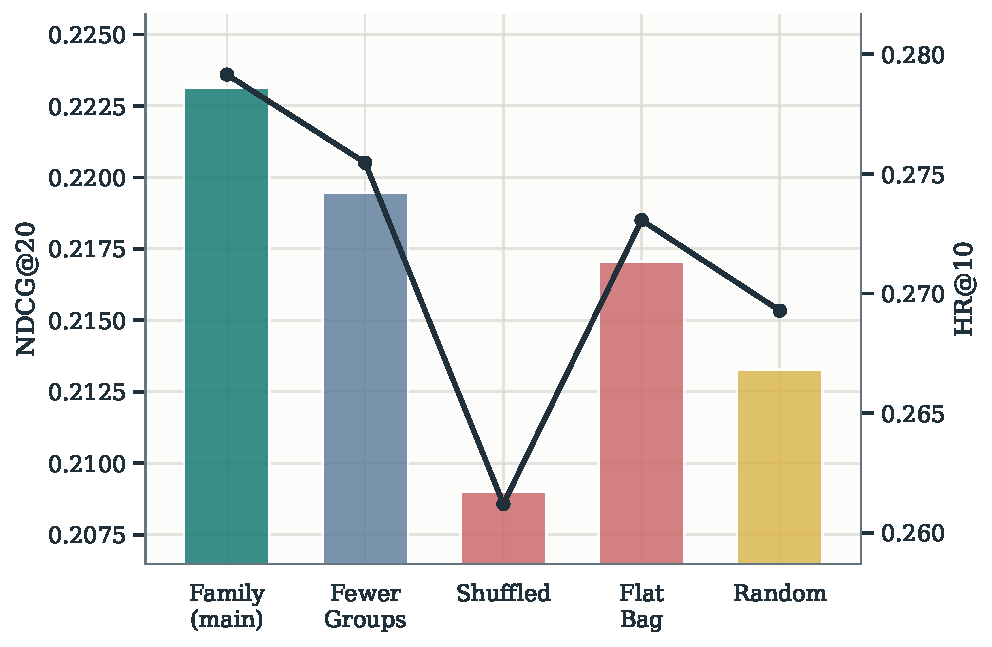
\includegraphics[width=\linewidth]{figures/appendix/a02_structural_cue_org.pdf}
    \vspace{0.1em}
    {\footnotesize (a) Cue and family-group organization variants}
  \end{minipage}\hfill
  \begin{minipage}[t]{0.48\textwidth}
    \centering
    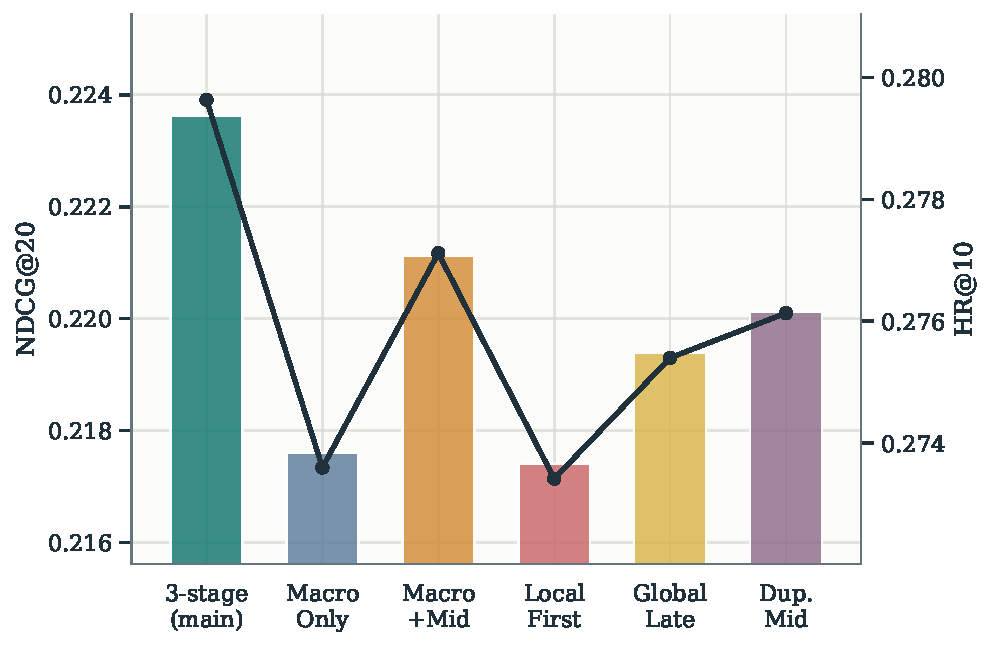
\includegraphics[width=\linewidth]{figures/appendix/a02_structural_temporal.pdf}
    \vspace{0.1em}
    {\footnotesize (b) Stage-semantics and temporal-layout variants}
  \end{minipage}
  \caption{Extended structural ablations. (a) Semantic cue and family-group organization variants. (b) Stage-semantics, temporal-role controls, and layout variants.}
  \Description{Two-panel figure for extended structural ablations: cue grouping variants and temporal layout variants.}
  \label{fig:appendix-stage-layout}
\end{figure*}

Panel (a) tests whether semantic grouping matters beyond a flat scalar bag. Panel (b) checks whether the macro, mid, and micro roles correspond to meaningfully distinct temporal views rather than just repeated copies of the same router, and whether the selected stage ordering remains the most stable high-performing layout among the temporal controls.

\section{Sparse Routing Design Variants}
\label{app:sparse-design}
Table~\ref{tab:appendix-sparse-design} tests whether the selected sparse hierarchy is an arbitrary engineering choice or a meaningful part of the RouteRec design. This section directly supports Q3 and Q4 by contrasting dense routing, flat sparse controls, and hierarchical top-$k$ variants under comparable activation budgets.

\begin{table}[H]
  \centering
  \caption{Sparse routing design variants, ranging from a dense reference to progressively sparser hierarchical configurations under comparable total expert pools.}
  \label{tab:appendix-sparse-design}
  \footnotesize
  \setlength{\tabcolsep}{4pt}
  \begin{tabularx}{\columnwidth}{@{}>{\raggedright\arraybackslash}Xcc>{\raggedright\arraybackslash}X@{}}
    \toprule
    Variant & MRR@20 & Active experts & Observation \\
    \midrule
    Dense full mixture & 0.336 & 12 & Reference control \\
    Flat sparse top-$6$ & 0.335 & 6 & Same active count without hierarchy \\
    Top-$2$gr, top-$1$ex & 0.332 & 2 & Extremely sparse reference \\
    Top-$2$gr, top-$2$ex & 0.335 & 4 & Strong group commitment, tight capacity \\
    Top-$3$gr, top-$2$ex & \textbf{0.339} & 6 & \textbf{Selected main setting} \\
    Top-$4$gr, top-$2$ex & 0.337 & 8 & Weaker group commitment \\
    Top-$3$gr, top-$3$ex & 0.338 & 9 & Larger active-compute budget reference \\
    \bottomrule
  \end{tabularx}
\end{table}

The table separates three related questions: whether sparsity itself helps, whether hierarchy matters beyond a flat top-$k$ mask, and whether the selected main setting provides a reasonable balance between route commitment and active capacity.

\section{Objective and Regularization Variants}
\label{app:objective}
This table isolates whether the observed routing semantics depend primarily on the selected auxiliary objective or remain visible across objective variants. Table~\ref{tab:appendix-objective} reports ranking quality together with routing-stability indicators for each objective configuration, allowing the diagnostics in Appendix~\ref{app:diagnostics} to be read with the objective contribution accounted for.

\begin{table}[H]
  \centering
  \caption{Objective and regularization variants.}
  \label{tab:appendix-objective}
  \footnotesize
  \setlength{\tabcolsep}{4pt}
  \begin{tabularx}{\columnwidth}{@{}>{\raggedright\arraybackslash}XYYY@{}}
    \toprule
    Variant & MRR@20 & Neighbor JSD $\downarrow$ & Route-entropy var.\ $\downarrow$ \\
    \midrule
    No auxiliary loss & 0.333 & 0.148 & 0.094 \\
    KNN consistency only & 0.336 & 0.127 & 0.091 \\
    z-loss only & 0.337 & 0.136 & 0.083 \\
    Balance loss only & 0.334 & 0.141 & 0.090 \\
    Consistency + z-loss & 0.338 & 0.124 & 0.080 \\
    Full objective & \textbf{0.339} & \textbf{0.121} & \textbf{0.079} \\
    \bottomrule
  \end{tabularx}
\end{table}

The two central comparisons are whether the selected objective improves ranking under sparse routing, and whether removing specific auxiliary terms materially changes the sharpness and consistency patterns reported in Appendix~\ref{app:diagnostics}.

\section{Full Cost and Efficiency Summary}
\label{app:efficiency}
Table~\ref{tab:appendix-efficiency} provides a compact cost summary for the claim that the routing branch is lightweight. Rather than turning the appendix into a systems study, this section reports the rough parameter and runtime overhead for representative baselines together with RouteRec's active-parameter view under sparse routing.

\begin{table}[H]
  \centering
  \caption{Model cost and efficiency summary for all compared methods.}
  \label{tab:appendix-efficiency}
  \scriptsize
  \setlength{\tabcolsep}{3pt}
  \renewcommand{\arraystretch}{1.05}
  \begin{tabularx}{\columnwidth}{@{}L{0.19\columnwidth}ccccL{0.32\columnwidth}@{}}
    \toprule
    Model & Params & Active params & Train $\times$ & Infer $\times$ & Note \\
    \midrule
    GRU4Rec & 1.4 & 1.4 & $0.83\times$ & $0.88\times$ & \makecell[l]{Dense recurrent reference} \\
    SASRec & 1.8 & 1.8 & $1.00\times$ & $1.00\times$ & \makecell[l]{Normalization anchor} \\
    TiSASRec & 2.1 & 2.1 & $1.31\times$ & $1.22\times$ & \makecell[l]{Time-aware Transformer} \\
    DuoRec & 2.0 & 2.0 & $1.28\times$ & $1.15\times$ & \makecell[l]{Contrastive sequential} \\
    FEARec & 2.0 & 2.0 & $1.35\times$ & $1.24\times$ & \makecell[l]{Frequency-aware} \\
    BSARec & 1.9 & 1.9 & $1.18\times$ & $1.10\times$ & \makecell[l]{Structural sequential} \\
    FAME & 2.8 & 2.8 & $1.62\times$ & $1.48\times$ & \makecell[l]{Expert-based baseline} \\
    DIF-SR & 2.4 & 2.4 & $1.42\times$ & $1.32\times$ & \makecell[l]{Feature-aware sequential} \\
    FDSA & 2.3 & 2.3 & $1.38\times$ & $1.28\times$ & \makecell[l]{Feature-side attention} \\
    RouteRec & 3.2 & 1.6 & $1.42\times$ & $1.18\times$ & \makecell[l]{Active params: routed subset only} \\
    \bottomrule
  \end{tabularx}
\end{table}

A compact cost comparison is sufficient here to anchor the selective-activation claim and to show that the observed gains are not being attributed solely to an unchecked increase in compute. The timing numbers in this table are measured on a single NVIDIA RTX 3090 24\,GB GPU under the same batch-size and evaluation conditions; the ratios serve as a practical reference point rather than as a deployment-grade systems benchmark.

\section{Extended Routing Diagnostics}
\label{app:diagnostics}
This section summarizes the final model's routing structure through aggregate diagnostics rather than controlled perturbations; targeted interventions are deferred to Appendix~\ref{app:qualitative-cases}. Figure~\ref{fig:appendix-diagnostics} groups the main diagnostics so that group usage, route sharpness, and stage-wise consistency can be read together. Together with the main-text cases, these plots provide the aggregate support for Q5.

\begin{figure}[H]
  \centering
  \begin{minipage}[t]{0.48\linewidth}
    \centering
    
\includegraphics[width=\linewidth]{figures/appendix/a03_routing_heatmaps.pdf}
    \vspace{0.1em}
    {\footnotesize (a) Stage-wise family and expert usage heatmaps}
  \end{minipage}\hfill
  \begin{minipage}[t]{0.48\linewidth}
    \centering
    
\includegraphics[width=\linewidth]{figures/appendix/a03_routing_diagnostics_lines.pdf}
    \vspace{0.1em}
    {\footnotesize (b) Route entropy and effective-expert-count summary}
  \end{minipage}
  \caption{Routing diagnostics. (a) Group/expert usage heatmaps by stage. (b) Route entropy and effective expert count across variants. Targeted intervention results are reported separately in Appendix~\ref{app:qualitative-cases}.}
  \Description{Two-panel figure showing routing diagnostics: usage heatmaps and route entropy summaries.}
  \label{fig:appendix-diagnostics}
\end{figure}

These diagnostics are organized from coarse structure to semantic interpretation. Panel (a) shows how family and expert usage is distributed by stage, while Panel (b) summarizes route sharpness and effective expert usage across the main sparse-routing variants.

\section{Extended Behavioral Slice Results}
\label{app:behavior-slices}
Unlike Appendix~\ref{app:special-bins}, which analyzes coarse difficulty-oriented bins, this section examines semantically defined behavioral regimes such as repeat-heavy, fast exploratory, narrow-focus, and preference-stable slices. It first defines the diagnostic slices explicitly, then extends the main-text regime analysis with per-dataset breakdowns and more detailed routing summaries.

\begin{table}[H]
  \centering
  \caption{Diagnostic slice definitions used in the behavior-regime analysis.}
  \label{tab:appendix-slice-definitions}
  \scriptsize
  \setlength{\tabcolsep}{4pt}
  \begin{tabularx}{\columnwidth}{@{}lX@{}}
    \toprule
    Slice & Definition rule \\
    \midrule
    Repeat-heavy & Prefix repeat ratio above a fixed percentile threshold \\
    Fast-tempo & Mean inter-event gap below a fixed percentile threshold \\
    Narrow-focus & Category or item-transition entropy below a fixed percentile threshold \\
    Exploration-heavy & Novel-item or low-repeat ratio above a fixed percentile threshold \\
    \bottomrule
  \end{tabularx}
\end{table}

These slices are used only for post hoc diagnosis. They are computed from simple observable statistics of the interaction history, not from optimized supervision targets, and not from labels learned jointly with the model.

\begin{figure}[H]
  \centering
  \begin{minipage}[t]{0.58\linewidth}
    \centering
    
\includegraphics[width=\linewidth]{figures/appendix/a04_behavior_slices.pdf}
    \vspace{0.1em}
    {\footnotesize (a) Slice-wise MRR@20 across behavioral regimes}
  \end{minipage}\hfill
  \begin{minipage}[t]{0.38\linewidth}
    \centering
    
\includegraphics[width=\linewidth]{figures/appendix/a04_slice_relative_gain.pdf}
    \vspace{0.1em}
    {\footnotesize (b) Relative RouteRec gain by slice}
  \end{minipage}
  \caption{Extended behavior-regime analysis. (a) Slice-wise ranking quality across behavioral regimes. (b) Relative RouteRec gain over SASRec by behavioral slice.}
  \Description{Two-panel figure for slice-wise MRR@20 and relative RouteRec gain across behavioral regimes.}
  \label{fig:appendix-behavior-slices}
\end{figure}

Together, the two panels expose dataset-level heterogeneity that would be too detailed for the main paper while making the slice construction explicit enough to avoid circular interpretation.

\FloatBarrier

\section{Targeted Interventions and Qualitative Cases}
\label{app:qualitative-cases}
This section complements the main-text case visualizations with controlled cue-family perturbations and directly inspectable qualitative examples. The main text presents three representative cases; the appendix adds a preference-stable contrastive case and the matched intervention evidence. Together, the intervention panels and the case table make the Q5 semantic claim readable at both the distribution level and the level of individual sessions.

\begin{figure}[H]
  \centering
  \begin{minipage}[t]{0.48\linewidth}
    \centering
    
\includegraphics[width=\linewidth]{figures/appendix/a05_intervention_score_drop.pdf}
    \vspace{0.1em}
    {\footnotesize (a) Score drop by cue-family perturbation}
  \end{minipage}\hfill
  \begin{minipage}[t]{0.48\linewidth}
    \centering
    
\includegraphics[width=\linewidth]{figures/appendix/a05_routing_profiles.pdf}
    \vspace{0.1em}
    {\footnotesize (b) Stage-wise routing profiles by behavioral case}
  \end{minipage}
  \caption{Targeted intervention analysis. (a) Score drop under cue-family perturbation for each behavioral regime. (b) Stage-wise routing profiles for the representative behavioral cases.}
  \Description{Two-panel figure showing intervention score drops and routing profiles by behavioral case.}
  \label{fig:appendix-interventions}
\end{figure}

\begin{table}[H]
  \centering
  \caption{Representative qualitative routing cases. Selected groups and experts are post hoc observations from the final model's routing decisions on each case type.}
  \label{tab:appendix-qualitative-cases}
  \tiny
  \setlength{\tabcolsep}{2pt}
  \renewcommand{\arraystretch}{1.05}
  \begin{tabularx}{\columnwidth}{@{}L{0.15\columnwidth}L{0.24\columnwidth}L{0.19\columnwidth}L{0.19\columnwidth}L{0.18\columnwidth}@{}}
    \toprule
    Case & Prefix summary & Selected groups & Prediction outcome & Interpretation \\
    \midrule
    Repeat-heavy & High repeat ratio; low inter-event variance; stable category distribution & Memory (macro, micro); Tempo (macro) & Correct revisit prediction; MRR$\approx$0.41 & Macro and micro routes reinforce revisit behavior \\
    Fast exploratory & Short inter-event gaps; high switch rate; low category entropy & Tempo (micro); Exposure (macro, mid) & Reasonable exploration target; MRR$\approx$0.35 & Micro routing sharpens under short-horizon volatility \\
    Narrow-focus & High dominant-group mass; low entropy; few distinct categories & Focus (mid, micro); Memory (macro) & Category-consistent recommendation; MRR$\approx$0.39 & Mid-stage routing concentrates on coherent intent \\
    Preference-stable & Long history; low recency drift; uniform pace & All groups near uniform; low route entropy & Moderate improvement over SASRec & Gains narrow when routing demand is weak \\
    \bottomrule
  \end{tabularx}
\end{table}

The intervention panels explain which semantic families the router appears to rely on most, while Table~\ref{tab:appendix-qualitative-cases} complements that distribution-level view with directly inspectable cases.

\FloatBarrier

\section{Optional Transfer Results}
\label{app:transfer}
This section reports optional transfer-style results examining whether RouteRec's portable routing interface can be reused across domains with different behavioral and temporal characteristics. The source-target matrix and low-resource curves provide the pairwise and data-efficiency views omitted from the main text.

\begin{figure}[H]
  \centering
  
\includegraphics[width=0.92\columnwidth]{figures/appendix/a06_transfer.pdf}
  \caption{Transfer analysis. Low-resource MRR@20 curves across data fractions comparing full fine-tune, finetuned router, anchor transfer, frozen router, and no-transfer baselines.}
  \Description{Figure showing low-resource transfer curves and transfer-strategy comparisons.}
  \label{fig:appendix-transfer-panels}
\end{figure}

Figure~\ref{fig:appendix-transfer-panels} shows how the routing interface transfers across data-efficiency regimes. Full fine-tuning and finetuned-router transfer consistently outperform the no-transfer baseline, while the frozen-router setting remains a lightweight alternative at higher data fractions.

\end{document}
